% $Id: GMAT-Architectural-Specification.tex,v 1.34 2007/12/21 17:00:37 dconway Exp $
\documentclass[letterpaper,10pt]{book}

\usepackage[T1]{fontenc}
\usepackage[latin1]{inputenc}
\usepackage{geometry}
\usepackage{graphics,color}
\usepackage{overcite}
\geometry{letterpaper}

% Used to customize captions
\usepackage[pointedenum]{paralist}

% Enable indexing
\usepackage{makeidx}
\makeindex

%  for showing script lines as they appear in GMAT
\usepackage{verbatim}

% Allows alignment of multiple columns of text
\usepackage{array}

% Enables text wrapping around small tables and figures
\usepackage{float}

% Enables text wrapping around small tables and figures
\usepackage{floatflt}

% Enables side by side figures
\usepackage[countmax]{subfloat}

% Enables line numbering for verbatim text
\usepackage{lineno}

% Some text listing help for script files
\usepackage{listings}
\lstset{frame=single, captionpos=b, language=Matlab, xleftmargin=36pt, xrightmargin=36pt,
basicstyle=\ttfamily, numberstyle=\tiny, numbers=none}

% Use special characters defined by the ams
\usepackage{amsmath}

% Allow rotating figures
\usepackage{lscape}

% Enable verbatiminput so functional script files can be read in directly
\usepackage{fancyvrb}

% Fixes some font sizing problems
\usepackage{fix-cm}

%  for making index, using landscape mode, for multi page tables, supertabular??
% This package is needed to include the tables in the GMATDocuments/common subfolder
\usepackage{longtable, supertabular}

%\usepackage{rotating}  %This breaks the png files in \includegraphics{} calls???

% Used for table organization
\usepackage{tabularx}

%\usepackage[listofnumwidth=5.5em]{subfig}

% Used to customize table and figure list spacings
\usepackage{tocloft}

% Used to customize captions
\usepackage{caption}

% for creating bookmarks in the final pdf file when using dvipdfm
\usepackage[dvipdfm, bookmarks = true, bookmarksopen]{hyperref}

%% Used to build enumerations of the form 1.2.3.4.  etc.
%\usepackage[pointedenum]{paralist}

% If going through postscript to pdf, use the following instead for bookmarks:
%\usepackage[dvips, bookmarks = true, bookmarksopen]{hyperref}

%% Used to build the glossary and acronym definitions
%\usepackage[toc]{glossaries}

% Construct the basic page sizes
\oddsidemargin  0.0in
\evensidemargin 0.0in
\textwidth      6.5in
\headheight     0.25in
\topmargin      0.0in
\textheight=8.5in

% Note that png and jpg extensions are used for graphics
\DeclareGraphicsExtensions{.png,.jpg}

%% The following lines customize spacing on the tables of contents, list of figures, etc.
% More space for figure numbers
\setlength{\cftfignumwidth}{3em}
% Space between elements of the list
%\setlength{\cftbeforefigskip}{0.1cm}
% Space before chapter entries in the TOC
%\setlength{\cftbeforechapskip}{0.2cm}
% Space before parts in the TOC
%\setlength{\cftbeforepartskip}{0.7cm}

%\setlength{\emergencystretch}{6em}
%\pretolerance=10000
%\tolerance=10000

%\define@key{caption}{listofnumwidth}[4em]{\def\sf@numwidth{#1}}


%-------------------------------------------------------------------------------
%------------------------------------New Commands-------------------------------
%-------------------------------------------------------------------------------
\newcommand{\st}[1]{\begin{ttfamily}#1\end{ttfamily}}
\newcommand{\boldst}[1]{\begin{ttfamily}\textbf{#1} \end{ttfamily}}
\newcommand{\br}[0]{$\mathbf{r} $}
\newcommand{\bv}[0]{$\mathbf{v} $}
\newcommand{\ba}[0]{$\mathbf{a} $}
\newcommand{\mbr}[0]{\mathbf{r} }
\newcommand{\mbv}[0]{\mathbf{v} }
\newcommand{\mba}[0]{\mathbf{a} }

%-------------------------------------------------------------------------------
%------------------------------------New Environments---------------------------
%-------------------------------------------------------------------------------

\newenvironment{ScriptType}
  {\noindent \begin{ttfamily}}
   { \end{ttfamily} }

\newenvironment{Script}
 { \vspace{-.15 in} \begin{ttfamily} }
 { \end{ttfamily}\vspace{-.25 in} }

% Turned off the watermark for now because it's annoying in proof mode
% Make the watermark
\usepackage{eso-pic}
\usepackage{color}
\usepackage{type1cm}
%\makeatletter
%  \AddToShipoutPicture{%
%    \setlength{\@tempdimb}{.5\paperwidth}%
%    \setlength{\@tempdimc}{.5\paperheight}%
%    \setlength{\unitlength}{1pt}%
%    \put(\strip@pt\@tempdimb,\strip@pt\@tempdimc){%
%      \makebox(0,0){\rotatebox{45}{\textcolor[gray]{0.75}{\fontsize{2cm}{2cm}\selectfont{Draft:
%Work in Progress}}}}
%    }
%} \makeatother

% Disabled for intermediate versions -- TURN ON FOR RELEASE VERSIONS
%\makeatletter
%  \AddToShipoutPicture{%
%    \setlength{\@tempdimb}{.5\paperwidth}%
%    \setlength{\@tempdimc}{.5\paperheight}%
%    \setlength{\unitlength}{1pt}%
%    \put(\strip@pt\@tempdimb,\strip@pt\@tempdimc){%
%      \makebox(0,675){\rotatebox{0}{\textcolor[gray]{0.75}{\fontsize{1.5cm}{1.5cm}\selectfont{Draft:
% Work in Progress}}}}
%    }
%} \makeatother

% Not currently using glossaries package
%% Commands used to generate glossary and acronym tables
%\newglossary{definitions}{def}{dfn}{GMAT Nomenclature}
%\makeglossaries

% Float style for script files and snippets
\floatstyle{boxed}
\newfloat{script}{htb}{scr}[chapter]
\floatname{script}{Script}

\setcounter{secnumdepth}{3}

%-------------------------------------------------------------------------------
%------------------------------------Begin The Doc!!----------------------------
%-------------------------------------------------------------------------------
\begin{document}

%  Here we define the style for the bib.
\bibliographystyle{aiaa}
\thispagestyle{empty}

%%------------------------------------------------------------
%%-----------------Cover Page and TOC-------------------------
%%------------------------------------------------------------


\vspace{2 in}

\begin{center}
{\renewcommand{\thefootnote}{\fnsymbol{footnote}} { \Huge \bf
Preliminary Design for OD in  the General Mission Analysis Tool
(GMAT): User Interfaces, Models, and Architecture. }}
\end{center}
\begin{center}
{\renewcommand{\thefootnote}{\fnsymbol{footnote}} { \Huge \bf
 DRAFT }}
\end{center}

\vspace{1 in}

\begin{center}
{\renewcommand{\thefootnote}{\fnsymbol{footnote}} { \large
 Darrel J. Conway\\
  Steven P. Hughes\\
  Thomas M. Kelecy\\
 Mathew P. Wilkins\\
 \normalsize \vspace{.5 in}
 \today
  }}
\end{center}




\clearpage \mbox{}\clearpage


\tableofcontents

\chapter{Introduction}

This document contains a high level description of intended orbit
determination features for the General Mission Analysis Tool (GMAT).
The document contains two fundamental types of information:  how the
user would interact with GMAT to perform orbit determination, and a
high level view of how GMAT will solve orbit determination problems.
The user perspective is documented by discussing components in GMAT
that would  enable OD applications and through use cases that
suggest how components may be configured to solve common OD
problems.    The system perspective is documented by describing the
system components GMAT will employ to perform OD and how these
components interact including activity diagrams, sequence diagrams
and important classes and methods.

At the time of this writing, the General Mission Analysis Tool
(GMAT) does not support estimation of orbit or attitude related
data.   This document is the product of an intensive design session
performed at AFRL/RDSM in Maui with the goal to determine high level
user interface and architectural design specifications for new
estimation capabilities.   Our goals for the 8 day meeting were:

1)  Define high level functionality and detailed use cases 2)
Identify major system components:  objects, commands, and
application control 3)  Describe how components interact to solve
basic OD problems 4)  Identify priorities for development effort 5)
Continue development of prototype batch least squares functionality

Section 2 of this document  discusses how a user might interact with
GMAT to define and solve estimation problems.  This includes how to
configure estimators, how to define what quantities are to be
estimated and considered, and what measurements are to be included
in the estimation process.  For complex scenarios that involve
events, we propose a method for defining the event sequence so the
estimator can estimate their properties.  We also present an
approach for defining complex OD problems with smoothing and complex
measurement and solve for parameters.

Section three of this document is a system level perspective of how
identified features may be implemented in the system.  We identify
new system components and discuss how they interact to solve
estimation problems.    Finally, in section 4, we present a catalog
of use cases that describe the estimation problem to be solved and
illustrate how the user would configure GMAT to solve the problem.

\chapter{User Interfaces}
    
To solve OD problems in GMAT, a user will have to create and
configure many objects that model physical components involved in
the measurement process such as spacecraft, receivers, clocks,
transmitters and celestial objects to name a few.  A user will also
have to configure measurement models, provide truth data or define
simulation parameters, and configure numerical solvers to determine
the best state estimate. Below we discuss how the user will provide
these and other types of information to define and solve OD problems
in GMAT.  In a sense, this portion of the document is a  short
user's guide  written before developing the software. This approach
is useful in several ways: it defines how a user will interact with
GMAT and allows analysts to provide feedback on the interfaces
before the system is written, and it gives some insight into various
designs for the the underlying software architecture.

We begin this chapter with a high level view of OD from the
perspective of a user who needs to apply GMAT to orbit
determination. We provide a categorization of models and algorithms
that a user will have control over and explain the overall
philosophy of the user interface in GMAT.  The high level
categorization explains where in the GMAT script and GUI a user
would need to go to set various types of information such as
dynamics models, process noise parameters, and measurement models to
name a few.  Next, we provide a detailed view of the primary objects
and commands required for orbit determination in GMAT.  These
sections go into detail on what fields are on each objects, and what
commands would be employed for different types of analysis.

\section{Overview and Philosophy}

To uniquely define an orbit determination problem, a user must often
provide hundreds of pieces of information ranging from clock drift
parameters, process noise characteristics, spacecraft physical
properties, ground station properties, and atmospheric modelling
parameters to name just a few. This section explains how these
pieces of information will be organized in GMAT and the philosophy
behind the organization of the data.  The goal is to provide an
intuitive interface for orbit determination analysis and explain
where a user would go to set different types of data, and why the
choices have been made.

To explain the organization of models and data, we present several
levels of detail into the organization of data and models for orbit
determination applications.  The first level view all models and
data into six categories and explains how these groups interact in
the estimation process.  These high level categories are:
measurement participants, measurements, estimators, dynamics models,
commands, and output.  Here we present which types of data are set
on each object and model. For example, you learn where clock bias
information is located and where process noise information is
located.   The second level view we present a simple estimation
example using the proposed script language and walk you through each
step to set up a batch least squares problem for a spacecraft and
one ground station.  Finally, we present a reference section that
describes all field names and settings contained in the five
categories. For example, in the reference section, you learn the
script syntax to set process noise parameters, and the different
process noise models that are available.

Let's begin with a introductory user perspective on to the primary
system components used in orbit determination.

\subsection{Introduction to System Components and Philosophy}

In GMAT, the objects and models used for orbit determination
applications can be categorized into 6 groups:  measurement
participants, measurements, dynamics models, estimators, commands,
and output.  Below we describe each of these groups and the
philosophy and functionality for each category in turn.  Fig.~
\ref{Fig:ODOrganization} shows a listing of each category with a
list of objects in models in each category.  Items in bold are
objects in GMAT that can be created using the \st{Create} command.
For example, you can create a clock named ``GPSClock" by using the
lines \st{Create Clock GPSClock}. Items that appear in italics in
Fig.~\ref{Fig:ODOrganization} are setttings and models available on
the object below which they appear.  For example, on a receiver, you
can set attenuation and bore site parameters.   Let's now look at
measurement participants in more detail.\\

\begin{figure}[htbp!]
    \begin{center}
    \begin{picture}(270,350)
    \special{psfile=ODOrganization.eps
    hscale= 85 vscale= 85 hoffset = -130 voffset = -340}
    \end{picture}
    \end{center}
    \vspace{0.2 in}
    \label{Fig:ODOrganization}
    \caption{Intermediate Level View: Objects and Commands Data and Settings }
\end{figure}


%\begin{figure}[htbp!]
%    \begin{center}
%    \begin{picture}(270,150)
%    \special{psfile=ODObjects.eps
%    hscale= 85 vscale= 85 hoffset = -130 voffset = -440}
%    \end{picture}
%    \end{center}
%    \vspace{0.2 in}
%    \label{Fig:ODObjects}
%    \caption{High Level View: Objects and Commands for OD Applications }
%\end{figure}


\textit{Measurement Participants}\\

Measurement participants are modles of physical objects that
``participate" in the process of creating a measured quantity that
is related to the spacecraft state.  Examples of measurement
participants include spacecraft, ground stations, celestial objects.
Measurement particpants can be actively or passively involved in the
measurement process. In the case of celestial navigation, a star may
serve as a passive participant.  In the a two-way range measurement,
the participants may be a ground station and a spacecraft.

In GMAT, measurement participants are created and configured
separately from measurement models (which are discussed below).  For
example, if a user requires a Doppler measurement between say Hubble
and Canberra, they first configure a spacecraft to model Hubble, and
then they configure a ground station to model Canberra. Once the
Hubble and Canberra objects are configured, the user creates a
measurement object and configures it to create a Doppler measurement
between Hubble and Canberra.  The philosophy is that measurement
participants exist independently from the measurement process, e.g.,
a spacecraft exists and advances in time even when measurements are
not being taken.  In this way, the separation of measurement
participants and measurements is similar to what happens in the real
applications.\\

\textit{Measurements}\\

In orbit determination, observed quantities used in the estimation
process are measurements of some property of electromagnetic wave
propagation among participants in the measurement process.
\cite{GTDS:89}  GMAT contains many types of measurements as shown in
Fig. \ref{Fig:ODOrganization} including Ground Station, TDRSS, GPS,
Celestial Object and Crosslink measurements.  An orbit determination
analyst may want to process simulated measurements to determine the
achievable accuracy for a given set of measurements and tracking
data schedule.  Operationally, analysts use observed measurement
values to generate best estimates for the spacecraft state. In GMAT,
a measurement object supports all of these functions by the
providing the following data:  observed measurement values (whether
they are read from a file or simulated), the computed (or expected)
value of the measurement, and the measurement partial derivatives.

Measurement objects are quite complex as a large amount of
user-provided data is required to perform the functions described
above.  For observations, you must provide GMAT with the file
format, name, and location.  When there is more data on a file than
you wish to process, you must provide data editing criteria and
information on which measurement types to include.  For computation
of the expected value you must provide the model with participants
for the measurements and a propagator to use to advance the state of
the participants.  Finally, for simulated data you must provide an
participants and a propagator along with measurement error models
such as bias and noise.\\

\textit{Estimators}\\

GMAT contains several estimators including batch, sequential, and
initial orbit determination solvers.  These algorithms solve for a
state estimate by processing measurements generated by measurement
objects configured by the user.  Hence, you must provide a list of
all measurements to include in a particular estimation run.  In
addition, the solver object is where the user specifies which
parameters are to be treated as solve-for and consider quantities.
Further data that is provided on the solver object is shown in Fig.
\ref{Fig:ODOrganization} and includes process noise parameters and
convergence tolerances to name a few.

\subsection{Intermediate Level View of System Components}


%To configure a measurement model, the measurement participants must
%be created and appropriately configured.   Fields on the Measurement
%Model object allow the user to define many different types of
%measurements given the specified list of participants.   If observed
%measurements are available from a standard file format, the user
%configures the measurement Model to read data from the desired file.
%In this case, the user must set object Ids on the measuement
%participants to match the Ids on the measurement file.  GMAT uses
%the file format and measurement Ids to determine how computed values
%are to be calculated.
%


\verbatiminput{GSMeasurement.script}
\verbatiminput{BatchLeastSquares.script}
\verbatiminput{ExtendedKalmanFilter.script}

%Estimators
%
%The third component required for an estimation problem is a solver.
%The user will have many solvers to choose from including but not
%limited to
%
%?   Initial orbit determination ?   Batch (least squares, other) ?
%Filters (SRIF, EKF, UKF)
%
%In GMAT the solver is a relatively simple object compared to the
%measurement model and the measurement  participants.  The job of the
%solver is to query configured measurement models for the observed
%and computed values  and the partial derivatives  and use this
%information  to generate state estimates.  Hence,  the estimator in
%GMAT knows little about the details of the measurement model
%computations or the configurations of the participants.
%
%A sample script segment for a BatchLeastSquare he user will specify
%the SolveFor and Consider parameters on the estimator, along with
%what measurements they would like the solver to process.
%
%%Create BatchLeastSquares BLSE BLSI.Measurements = BLSI.Propagator =
%%BLSE.SolveFor = BLSE.Consider = BLSE.SolutionEpoch =
%%BLSE.AbsoluteConvergenceTol = BLSE.Propagator =
%%
%%Create ExtendedKalmanFilter EKF EKF.Measurements = EKF.Propagator =
%%EKF.SolveFor = EKF.Consider = EKF.SolutionEpoch = EKF.Propagator =
%%EKF.ProcessNoiseModel = EKF.Smoothing = Dynamics Models
%
%Dynamics Models ?   Participant dynamics ?   Variational equations ?
%Process Noise
%
%Commands and Application Control
%
%Application Control Modes ?   RunEstimator ?   SimulateData ?
%RunEstimatorSequence

    

\section{Particants}


\subsection{Spacecraft}

Receiver, Transmitter, Clock

\subsection{Ground Station}

\subsection{Space Network}

\subsection{GPS Constellation}

    \section{Measurements}

%When observed values are not available, a user can configure a
%Measurement Model to simulate the desired measurements.  In this
%case, GMAT will compute both the observed and expected values for a
%measurement, or by using the SimulateData command, GMAT will simply
%write the requirested simulation data to a measurement file.    A
%script snippet that contains a sample measurement model is shown
%below.  Each field for the Measurement Model object is discussed in
%detail in Table 1.  Note that for complex, such as GPS psuedorange,
%there will be many more fields.  These fields are not included here.
%
%Below is a script example of a simple measurement model.  The
%participants in the measurement are ODSat and Canberra, which are
%assumed to have been configured in a previous script segment.   The
%measurement types are Azimuth, Elevation, and Range.  The DataSource
%field allows the user to tell GMAT whether to read the observations
%from a file, or to simulate the data. The FileFormat and Filename
%fields allow the user to specify the observations data file if it is
%available.    The fields  LightTimeModel, IonosphericModel, and
%TroposphereModel,allow the user to specify the model for these error
%corrections, where None is an option if the error source is to be
%neglected.   All fields with the prefix field ".Sim" are for
%configuration of the data simulator for this measurement.

\subsection{Ground Station}

\subsection{GPS}

\subsection{TDRSS}

\subsection{Measurement Editing}

    \section{Solvers}

\subsection{Batch Least Squares}

\subsection{Extended Kalman Filter}

    \section{Estimation and Simulation}

    \section{Use Cases}

\subsection{Simple Batch Least Squares}

\subsection{Simple Extended Kalman Filter}

\subsection{Advanced SolverFor and Consider Parameters}

\subsection{Advanced Measurement Models}

\subsection{OD with Events}

\subsection{Measurement Simulation}

\subsection{Metric Calibration}

\subsection{Multiple Spacecraft Estimation}

\subsection{Non-Earth Estimation}

    \section{Output}


\chapter{Models and Mathematical Specifications}
    \section{Estimation State Vector}

Depending upon the application, GMAT may maintain  two types of
state vectors:  the propagation state vector and the estimation
state vector.  Here we define the propagation state vector to be the
set of components  the propagator component advances in time via
numerical integration or analytic propagation.  The estimation state
vector is defined as the vector of solve-for and consider parameters
associated with a particular estimator.

Elements in the propagation state vector may not be contained in the
estimation vector and vice-versa depending upon the particular
problem.  Managing and organizing state data presents a difficult
bookkeeping problem for several reasons

\begin{compactenum}
     \item Different state components may require different types of
     propagation methods.  (numerical integration vs. analytic
     or ephemeris interpolation)
     \item In GMAT, different spacecraft can be propagated by
     simulateously using different numerical integrators and
     force models.
     \item Propagation state data is not specified in one location.
     \item GMAT must maintain synchronous propagation if requested
     by the user.
     \item All components of propagation may not be known until
     runtime for a propagation command.
\end{compactenum}



\subsection{Orbit State}

\subsection{Dynamics Properties}

\subsection{Biases}

\subsection{Process Noise}

    \section{Propagation State Vector}

    \section{Dynamics}

    \chapter{The Estimators and Simulator}

\chapauthor{Stephen P. Hughes}{NASA/Goddard Space Flight Center}
\chapauthor{Darrel J. Conway}{Thinking Systems, Inc.}
\chapauthor{Matthew P. Wilkins}{Schafer Corporation}

GMAT's Estimator classes are shown in Figure~\ref{fig:EstimatorClasses}.  The first estimator build of GMAT includes the blocks shaded orange in the diagram: the Estimator base class, the BatchEstimator intermediate class, and the BatchLeastSquares estimator.  The second build adds the Filter intermediate class and a Kalman filter based estimator to the system.  Potential extensions to this class hierarchy are shown in the figure as well.

\begin{figure}[htbp]
\begin{center}
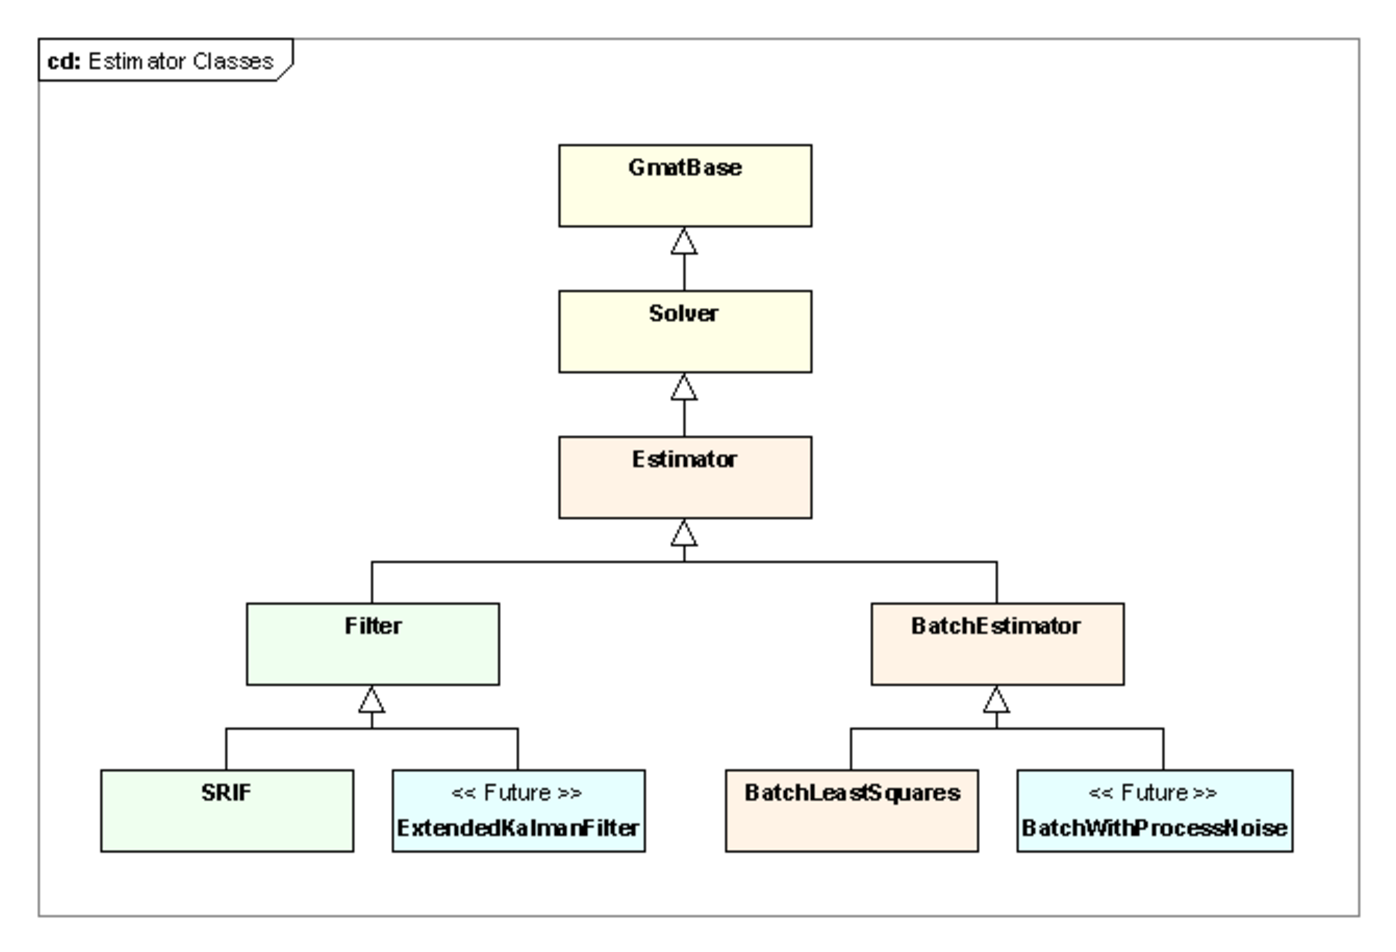
\includegraphics[scale=0.6]{Images/EstimatorClasses.eps}
\caption{\label{fig:EstimatorClasses}Classes in GMAT's Estimator Hierarchy}
\end{center}
\end{figure}

GMAT's Estimator base class defines the core functionality shared by all estimators.  It includes the top level Estimator interfaces, initialization code for the shared elements including the EstimationStateManager and MeasurementManager, and the member components implementing these elements.  The interfaces in this class are defined so that the estimation commands can treat the estimator process generically, and therefore drive the estimation process without intimate knowledge of the algorithm that is implemented in the estimator.

GMAT's estimator classes are derived from the Solver base class.  The Solver class provides data structures and methods designed so that derived classes can implement a finite state\footnote{``State'' in the context of a finite state machine corresponds to the status of the machine.  This is distinct from the state vector used by an estimator or SpaceObject.  When the context does not make the distinction clear, the term ``finite state'' is used for the state machine states and ``state vector'' for the data.} machine that, together with a matching command, organizes the process of working with the elements of the a GMAT mission to drive the algorithm implemented in the solver.  The command portion of this partnership manages the interface with the Sandbox and the propagation subsystem, and, when appropriate, with a solver control sequence designed to provide a sequence of commands when that sequence involves more than just direct propagation.  The solver side of the partnership manages the state of the solution algorithm.  That state is represented by one of several distinct values; hence the state machine is called a finite state machine.  The command side retrieves the state if the state machine from the solver, performs any necessary control sequence actions, and then passes control to the solver so that the solver can evaluate and potentially change state based on the results of the command's actions.

The state machine in GMAT's solvers provides a mechanism to ensure that the control sequence is executed in a sensible manner for the implemented algorithm.  As such, each derived solver class will define its state machine to meet the needs of its algorithm.  The state machines for each of the new estimators are described in the corresponding class descriptions below.

The following sections describe each estimation class in the figure, starting with the Estimator base class.  The capabilities and member elements are described, along with the processes that each class implements.

\section{The Estimator Base Class}

The Estimator class contains two key member objects used by all of GMAT's estimators: an instance of the EstimationStateManager and an instance of the MeasurementManager.  The details of those classes are provided in the corresponding sections of this document.  In this section you will see how these objects are set up and used by the Estimator classes.

Figure~\ref{fig:EstimatorClassDetails} shows the Estimator class, its ancestors, and its predecessor. The details of the class contents are shown in this figure, along with the helper classes mentioned above.  The Estimator class centralizes the interfaces to the measurement data and the estimation state vector, along with the other elements that all estimators need.  This class extends the features of the Solver class by adding and initializing these new elements.  As a base class, we anticipate that the implementation process for the derived estimators will result in a fair amount of refactoring, particularly as the BatchEstimator and Filter classes are implemented, consolidating additional common estimation features.

\begin{figure}[htbp]
\begin{center}
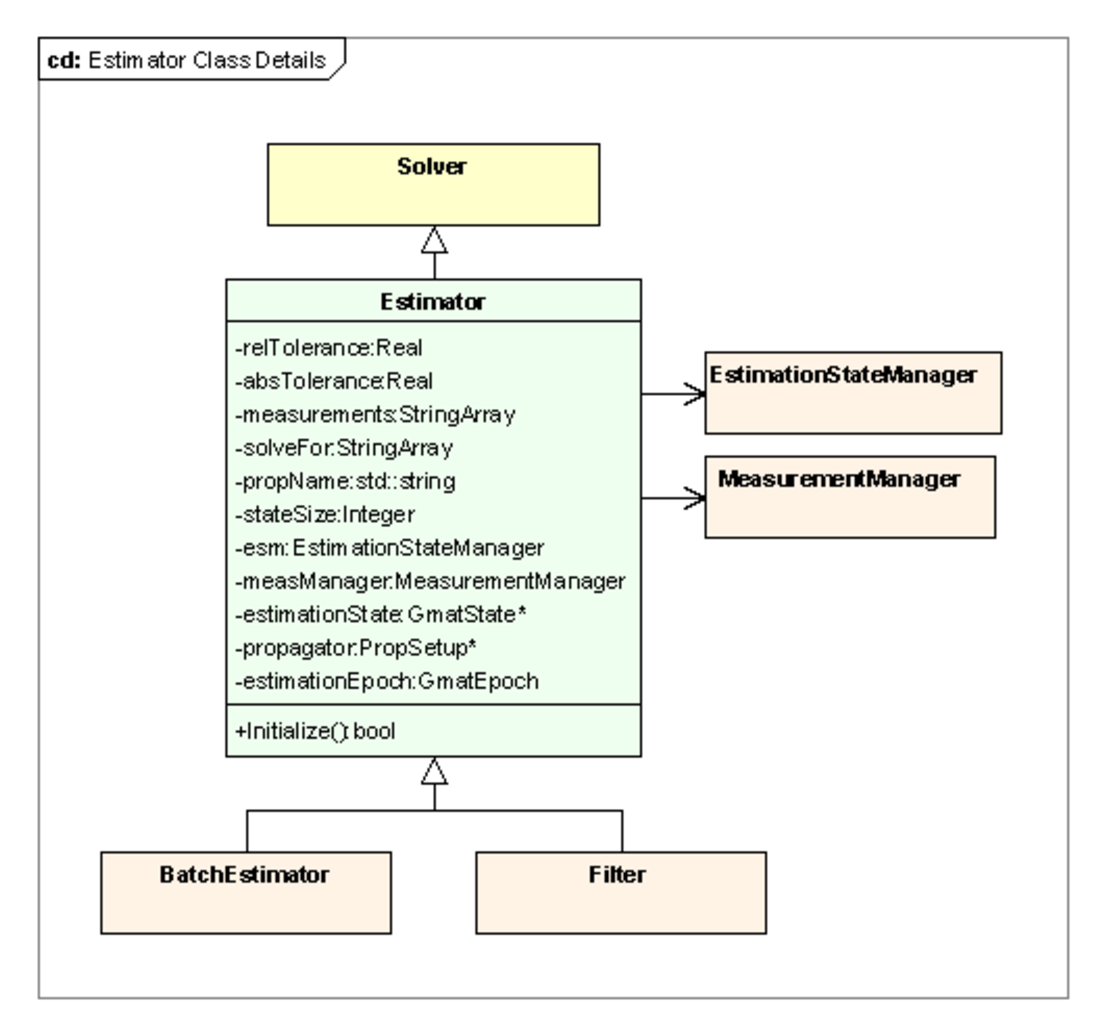
\includegraphics[scale=0.6]{Images/EstimatorClassDetails.eps}
\caption{\label{fig:EstimatorClassDetails}The Estimator Class}
\end{center}
\end{figure}

\subsection{Key Processes}

The Estimator base class has one key process: the Initialize method, which  initializes its management members and prepares its propagation subsystem for initialization.

\subsubsection{Estimator Initialization}

The Estimator class manages the initialization of the EstimationStateManager and the MeasurementManager, along with preparation of the PropagationStateManager for initialization, as is shown in Figure~\ref{fig:EstimatorInitialize}.  The Estimator::Initialize() method calls the Solver::Initialize() method first to ensure that the Solver data structures are properly prepared for use.  Following this call, the EstimationStateManager::Initialize() method is called, which sets the data structures for the estimation state vector and then builds the vector.  Once the estimation state vector has been built, the Estimator walks through the estimation state vector and passes each element that needs propagation into the PropagationStateManager assigned to the Estimator's propagator.  This process prepares the propagation subsystem for initialization, but does not perform the actual initialization.  That call is made in the estimation command immediately prior to execution so that all transient forces required for the propagation can be managed.  Finally, the MeasurementManager::Initialize() method is called, causing the measurement manager to read all of the data available for processing and to build the structures needed for that processing.  This step completes initialization for the Estimator base class.

\begin{figure}[htbp]
\begin{center}
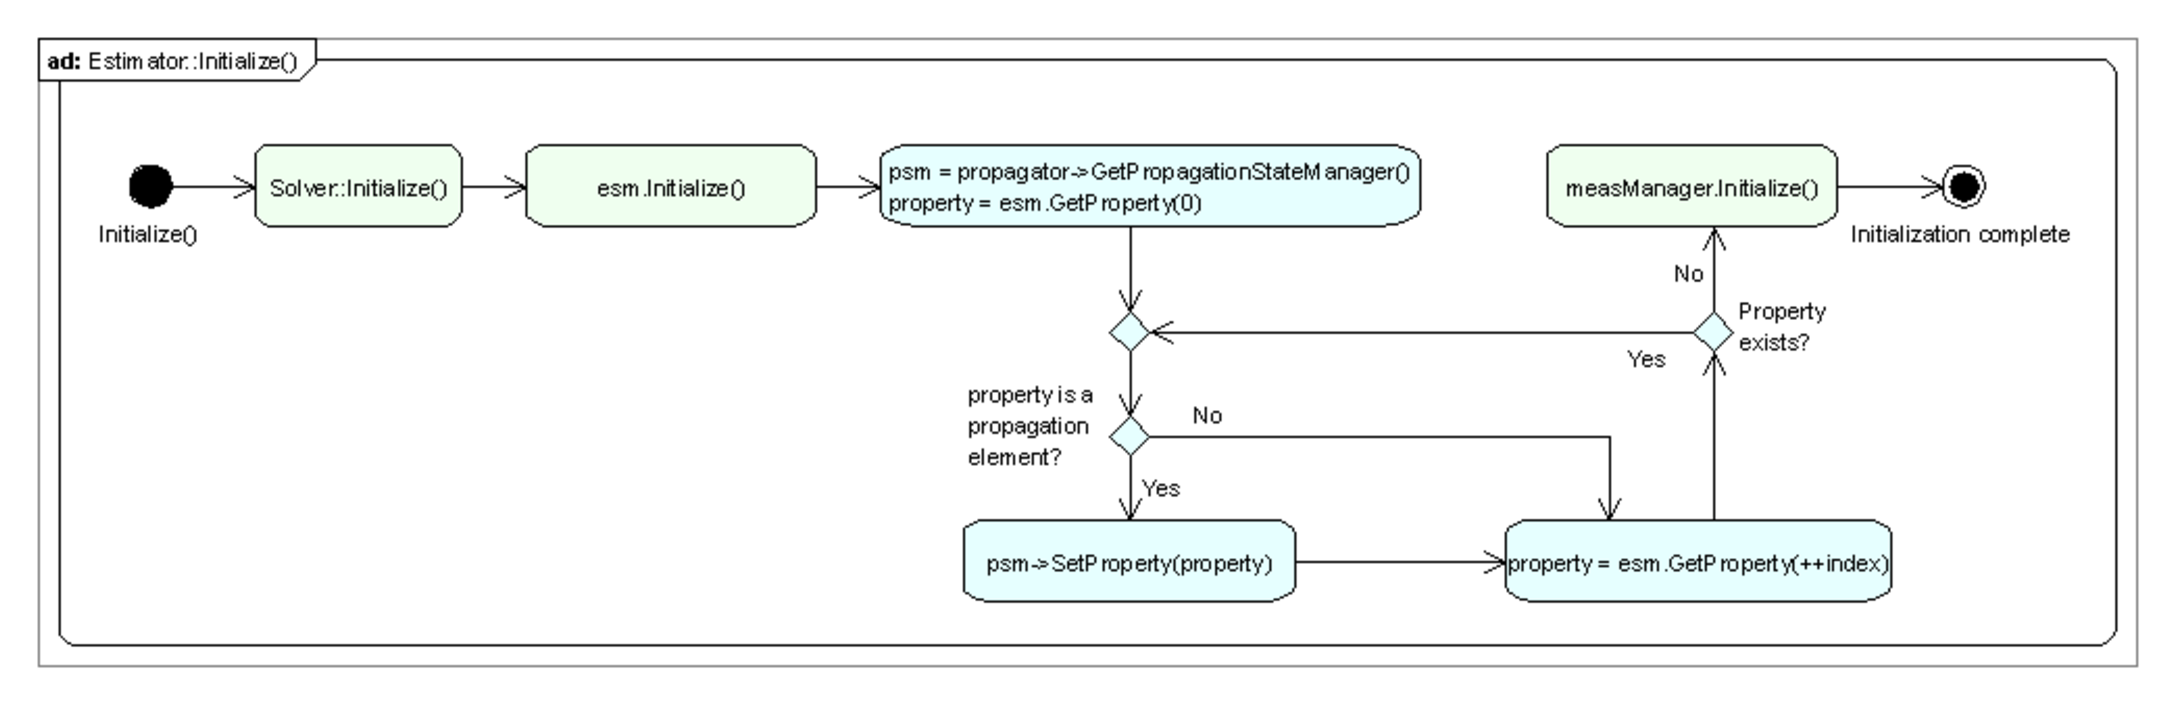
\includegraphics[scale=0.45]{Images/EstimatorInitialize.eps}
\caption{\label{fig:EstimatorInitialize}Estimator Class Initialization}
\end{center}
\end{figure}

\subsection{Estimator Members}

\paragraph{Estimator Attributes}

\begin{itemize}
\item \textbf{Real relTolerance}:  The maximum change from the previous RMS error in the residuals to the current RMS error allowed in order for convergence to be met.
\item \textbf{Real absTolerance}:  The largest allowed change in the estimation state in order for convergence to be met.
\item \textbf{StringArray measurements}:  Names of the measurement types used in this estimator.  This array of names is passed to the MeasurementManager for processing.
\item \textbf{StringArray solveFor}:  List of the solve for parameters used in the estimator.
\item \textbf{std::string propName}:  Name of the configured propagator used to evolve objects during the estimation process.
\item \textbf{Integer stateSize}:  The size of the estimation state vector.
\item \textbf{EstimationStateManager esm}:  The EstimationStateManager for the estimator.  This member is responsible for the communications between GMAT's objects and the data structures manipulated by the estimator during the estimation process.
\item \textbf{MeasurementManager measManager}:  The MeasurementManager for the estimator.  This object is responsible for managing all of the measurement objects in the estimation process.  It is an intermediary responsible for retrieving observed and calculated data, and supplying those data to the estimator.
\item \textbf{GmatState *estimationState}:  A pointer to the estimation state managed by the EstimationStateManager.  This pointer is set after the EstimationStateManager is initialized.  It is provided for convenience, so that repeated calls to esm.GetState() are not needed in the code.
\item \textbf{PropSetup *propagator}:  The propagator configured for the estimation.
\item \textbf{GmatEpoch estimationEpoch}:  The estimation epoch.  For batch estimators, this epoch is the epoch of the state estimate.  For sequential epochs, it tracks the epoch of the current estimate.
\end{itemize}

\paragraph{Estimator Methods}

\begin{itemize}
\item \textbf{bool Initialize()}:  Prepares the EstimationStateManager and MeasurementManager for use in estimation, and loads the propagator's PropagationStateManager so it can be initialized by the propagation enabled commands.
\end{itemize}

\section{The BatchEstimator Class}

\begin{figure}[htbp]
\begin{center}
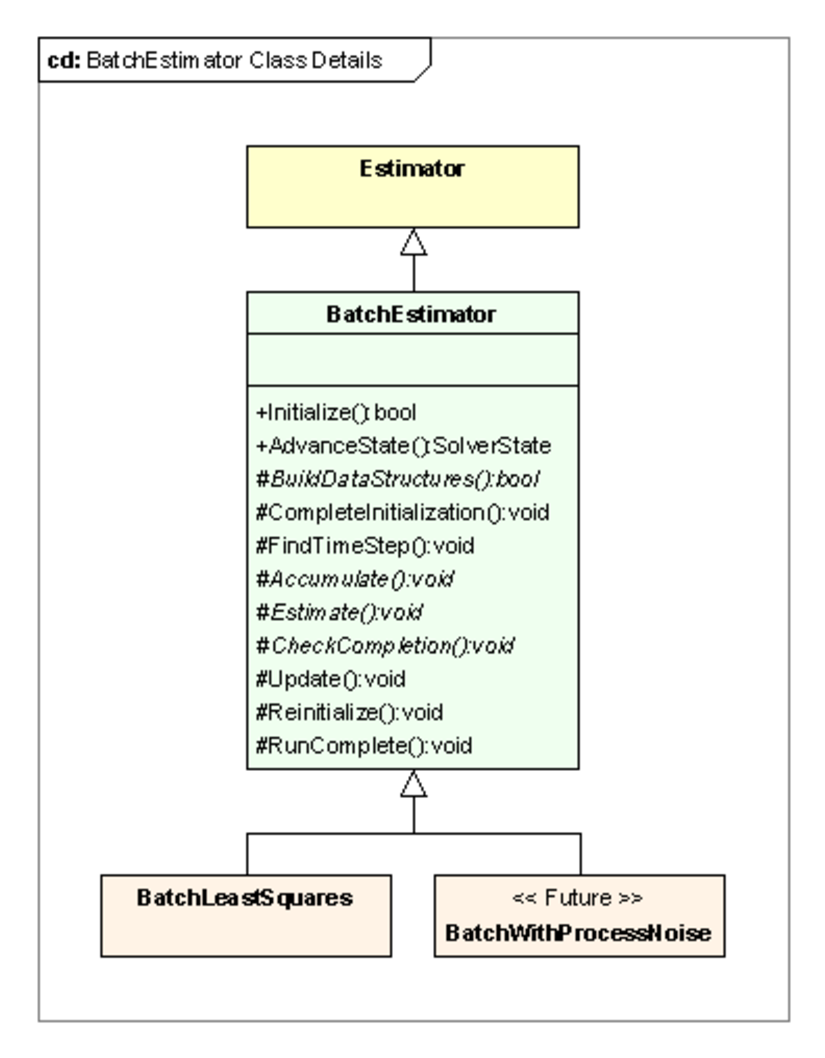
\includegraphics[scale=0.6]{Images/BatchEstimatorClassDetails.eps}
\caption{\label{fig:BatchEstimatorClassDetails}The BatchEstimator Class}
\end{center}
\end{figure}

The BatchEstimator class, shown in Figure~\ref{fig:BatchEstimatorClassDetails}, implements the infrastructure used by GMAT's batch estimators.  This infrastructure includes the implementation of a state machine intended to support the usual sequence of actions needed for batch estimation. The class defines with the methods called from this state machine, and provides implementations of the methods that are considered to be common to the batch estimation process.  All of the common methods implemented for the BatchEstimator class are declared virtual.  Derived classes can override the estimation state machine or any of the implemented methods as needed to support algorithm specific needs.  The Accumulate(), Estimate(), and CheckCompletion() methods are considered to always be implementation specific, and therefore must be implemented in the classes derived from the BatchEstimator class.

\subsection{Key Processes}

The BatchEstimator class implements a basic finite state machine that follows a typical batch estimation process.  There are two processes that work together to implement the state machine: initialization of the BatchEstimator and execution of the finite state machine.

\subsubsection{Initialization}

The initialization process in the Sandbox starts with the object setting phase described in the GMAT run overview.  At the end of this phase, all of the references objects have been set on the BatchEstimator object, and it is ready to validate those objects and set the pointers for use in the estimation process.  This process is shown in Figure~\ref{fig:BatchEstimatorInitialize}.

\begin{figure}[htbp]
\begin{center}
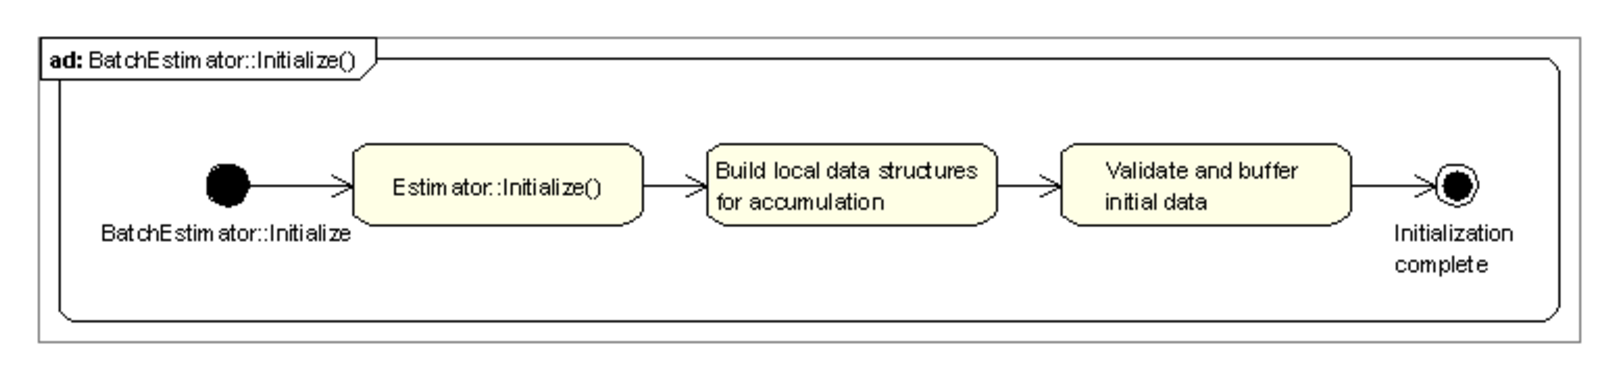
\includegraphics[scale=0.6]{Images/BatchEstimatorInitialize.eps}
\caption{\label{fig:BatchEstimatorInitialize}Initialization in the BatchEstimator Class}
\end{center}
\end{figure}

The initialization process for the BatchEstimator starts by initializing the Estimator base class as described above.  Once that process completes successfully, the data structures required for accumulation are prepared.  Finally, the initial data are checked to be sure that they contain all of the required data, and that these data are internally consistent, and they are buffered so they can be restored during iteration.  This completes the initialization process for the batch estimator.

\subsubsection{Estimation State Machine}

Figure~\ref{fig:BatchEstimatorOverview} shows the estimation process implemented in the BatchEstimator class.  The batch estimator state machine is shown in the lower partition in the figure, while the actions performed by the command running the state machine are shown in the upper partition.  The state machine implementation is key to the estimation process in GMAT, so it will be described in some detail in the following paragraphs.

\begin{figure}[htbp]
\begin{center}
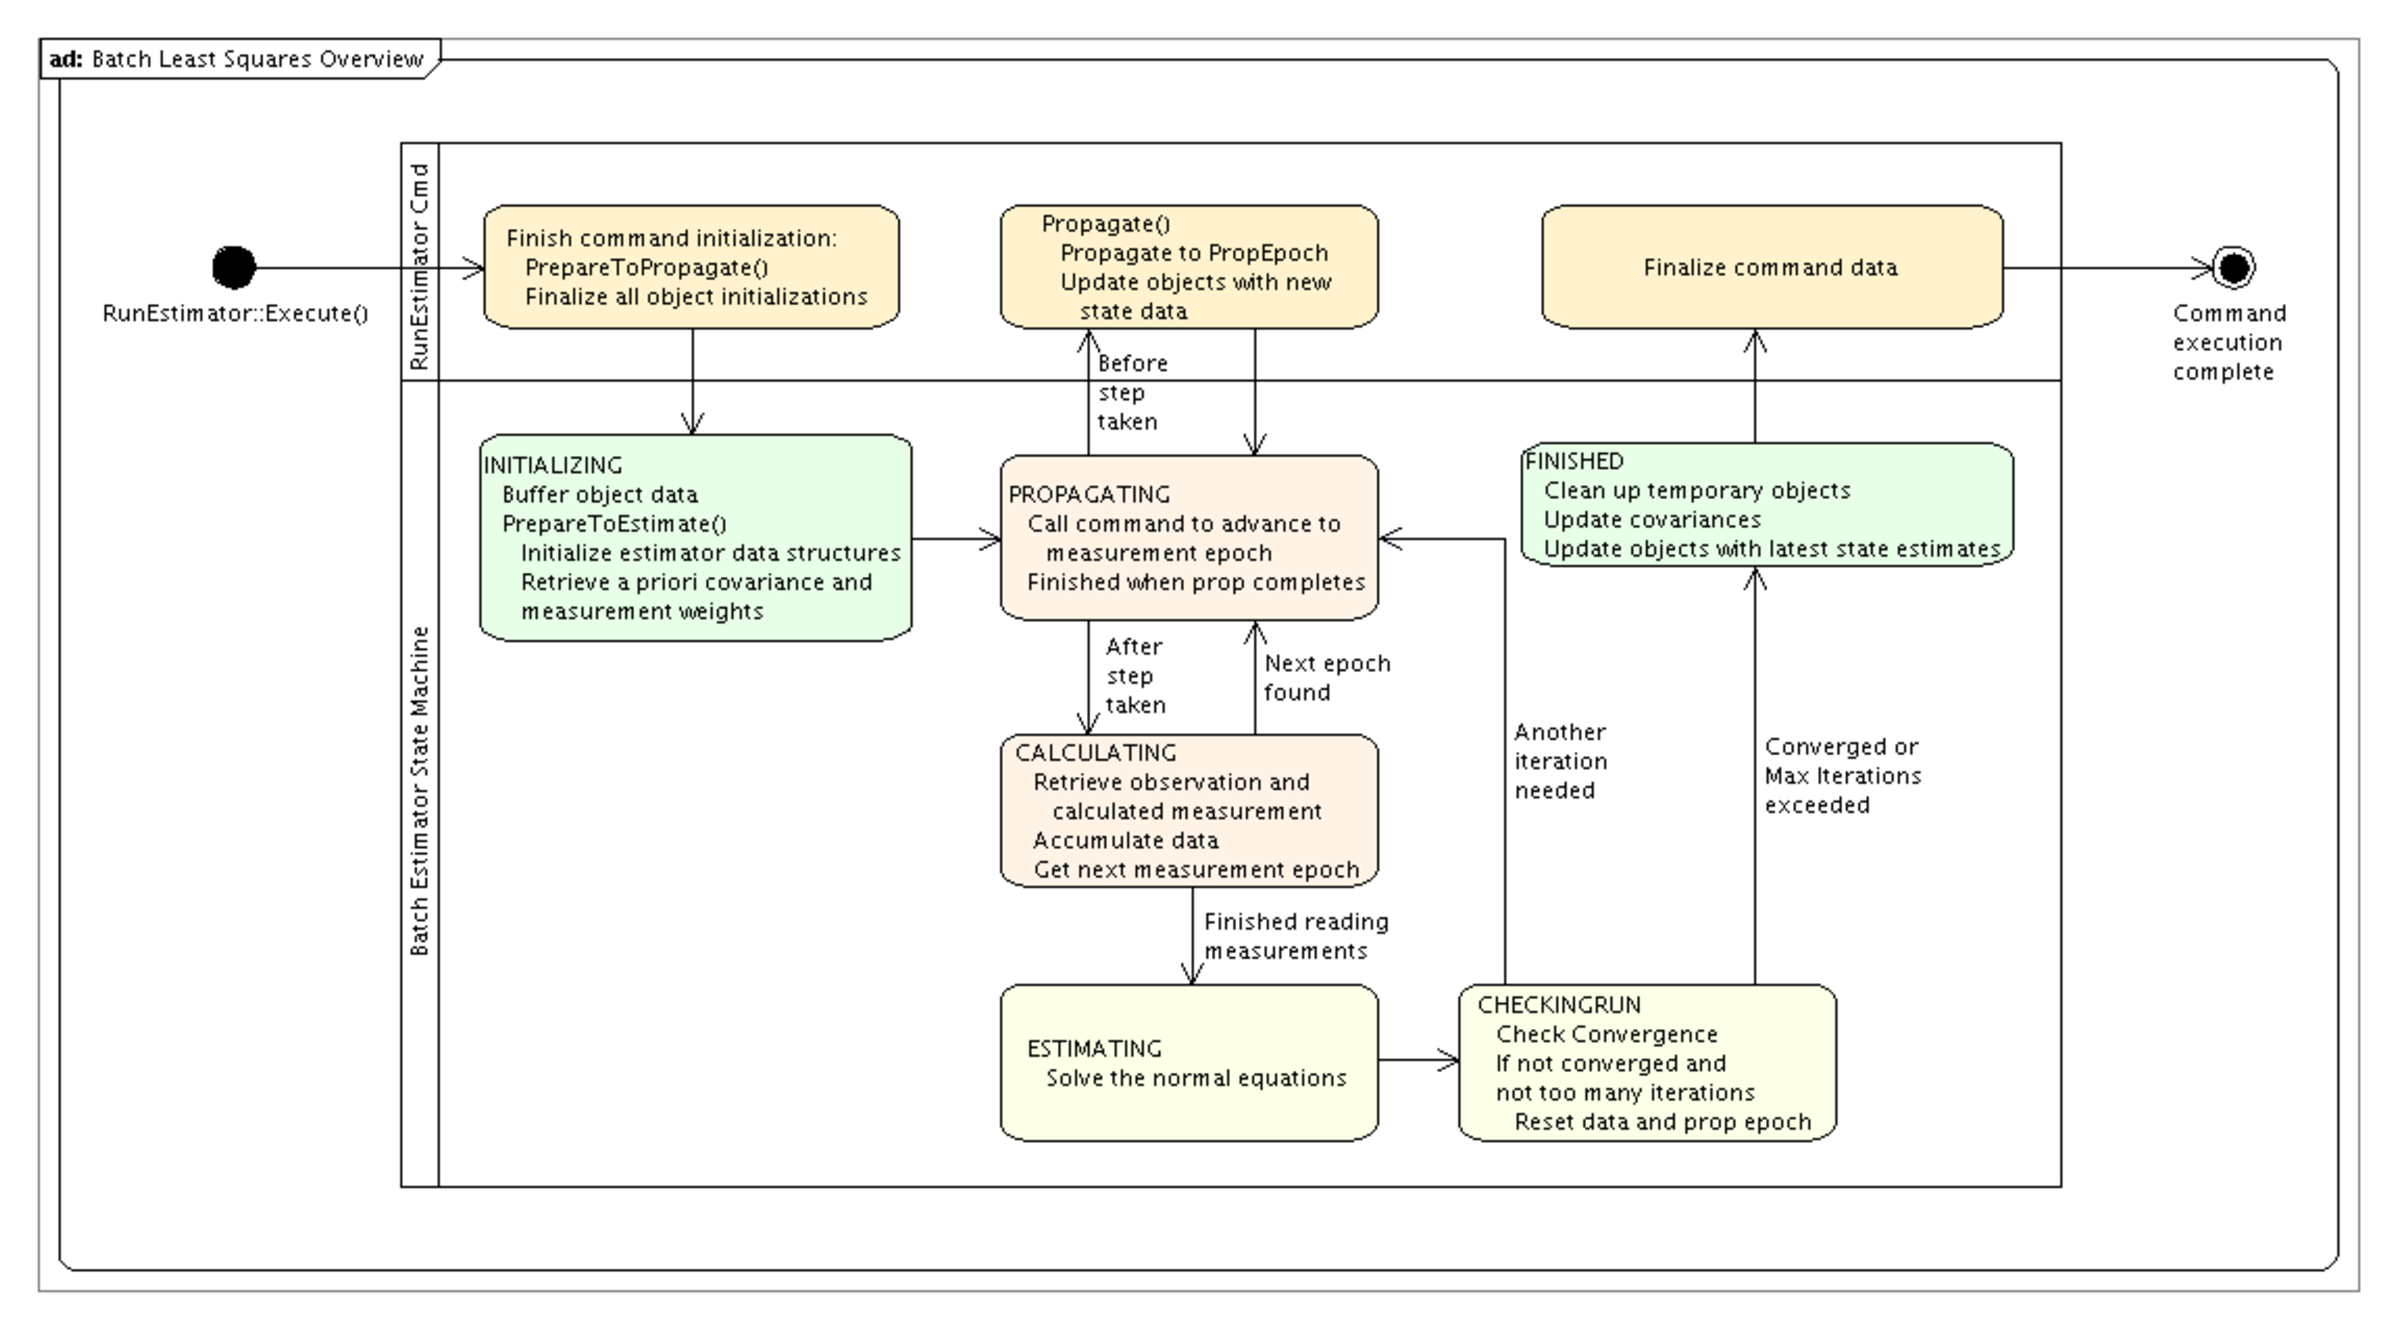
\includegraphics[scale=0.4]{Images/BatchLeastSquaresOverview.eps}
\caption{\label{fig:BatchEstimatorOverview}Performing Batch Estimation}
\end{center}
\end{figure}

\paragraph{GMAT's Solver State Machines}

GMAT's solver finite state machines are used to move the solution algorithm through the steps required to apply the algorithm to the objects that are used to solve a user specified problem. Each step of the process is represented by a discrete numerical identifier, referred to as the state of the process.  That identifier is used to specify a set of actions that, when performed, prepare the finite state machine to advance from its current state to the next state in the solution process.  The state identifiers are defined in a C++ enumeration, the SolverState enumeration in the Gmat namespace.

Each state in the solver state machine performs actions designed to move the elements of GMAT from their entry condition to the condition required to advance to the next state.  GMAT advances from one state to the next using the AdvanceState() method on the solver.  When AdvanceState() is called, the solver executes a method assigned to the state and reports the results to the solver's text file.  The method call is responsible for running the actions assigned to the state, and then determining the next state and changing the state identifier accordingly based on the results of the actions executed.

\paragraph{The BatchEstimator Finite State Machine}

The BatchEstimator uses seven states to drive its algorithm.  These seven states, shown in the bottom partition of Figure~\ref{fig:BatchEstimatorOverview}, work together to estimation a user defined state vector.  The list below describes each state of the machine, including the entry and exit conditions along with the internal actions required to move to the exit condition for the state:

\begin{description}
\item[INITIALIZING]\hspace{1pt}
\begin{itemize}
\item \textbf{Entry condition} The INITIALIZING state is the state the BatchEstimator takes upon completion of initialization in the Sandbox.  Upon completion of an estimation run, the BatchEstimator returns to this state so that a subsequent call can reuse the same estimator.
\item \textbf{Actions} \textit{Method Name: CompleteInitialization()}
\begin{itemize}
\item Determine if any observations are available; if not, abort estimation 
\item If necessary, propagate to estimation epoch
\item Gather the data and fill the batch estimator's state
\item Initialize the state transition matrix
\item Gather a priori covariances and measurement weights
\item Buffer all estimation objects
\end{itemize}
\item \textbf{Exit condition}
\begin{itemize}
\item Change to PROPAGATING state if an observation exists.  
\item Change to FINISHED state and post a warning message if none were found\footnote{The state machine in the figure shows the nominal path through the process.  Anomalous paths, like the absence of observation data mentioned here, are not included in the figure}.
\end{itemize}
\end{itemize}
\item[PROPAGATING]\hspace{1pt}
\begin{itemize}
\item \textbf{Entry condition}  An observation was found
\item \textbf{Actions} \textit{Method Name:  GetStepEpoch()}
\begin{itemize}
\item Determine time step for propagation to the observation epoch
\item Feed time step to command for propagation
\item Determine if measurement for the observation has events that require propagation
\end{itemize}
\item \textbf{Exit condition 1}
\begin{itemize}
\item Time step = 0
\item No unprocessed propagation events
\item Change state to CALCULATING
\end{itemize}
\item \textbf{Exit condition 2}
\begin{itemize}
\item Time step = 0
\item Events that require propagation not yet processed
\item Change state to LOCATING
\end{itemize}
\end{itemize}
\item[LOCATING]\hspace{1pt}
\begin{itemize}
\item \textbf{Entry conditions}
\begin{itemize}
\item An event that requires propagation has been found
\item Resources are at a known epoch for the event
\end{itemize}
\item \textbf{Actions} \textit{Method Name:  ProcessEvent(bufferData)}
\begin{itemize}
\item If bufferData is true, buffer state information
\item Calculate time step required for the event
\item Provide time step to command for propagation
\item Evaluate event to determine if propagation results are within tolerance
\item Iterate from time step calculation until event converges
\end{itemize}
\item \textbf{Exit condition 1}
\begin{itemize}
\item Event has converged
\item No additional events found
\item Reset state information to buffered data
\item Set bufferData flag to true
\item Change state to PROPAGATING
\end{itemize}
\item \textbf{Exit condition 2}
\begin{itemize}
\item Event has converged
\item Another event found
\item Set bufferData flag to false
\item Change state to LOCATING
\end{itemize}
\end{itemize}
\item[CALCULATING]\hspace{1pt}
\begin{itemize}
\item \textbf{Entry condition} Propagation and any required event location has been performed
\item \textbf{Actions} \textit{Method Name:  Accumulate()}
\begin{itemize}
\item Retrieve observation and calculated data
\item Accumulate the data
\item Retrieve the epoch of the next observation
\end{itemize}
\item \textbf{Exit condition 1}
\begin{itemize}
\item Another observation was found
\item Change state to PROPAGATING
\end{itemize}
\item \textbf{Exit condition 2}
\begin{itemize}
\item Final observation was processed
\item Change state to ESTIMATING
\end{itemize}
\end{itemize}
\item[ESTIMATING]\hspace{1pt}
\begin{itemize}
\item \textbf{Entry condition} All measurement data has been processed
\item \textbf{Actions} \textit{Method Name:  Estimate()}
\begin{itemize}
\item Solve the normal equations
\end{itemize}
\item \textbf{Exit condition}
\begin{itemize}
\item Estimation update generated
\item Change state to CHECKINGRUN
\end{itemize}
\end{itemize}
\item[CHECKINGRUN]\hspace{1pt}
\begin{itemize}
\item \textbf{Entry condition} An estimation update was generated
\item \textbf{Actions} \textit{Method Name:  CheckCompletion()}
\begin{itemize}
\item Check for convergence
\end{itemize}
\item \textbf{Exit condition 1}
\begin{itemize}
\item Estimation converged within tolerances
\item Change state to FINISHED
\end{itemize}
\item \textbf{Exit condition 2}
\begin{itemize}
\item Estimation did not converge
\item Maximum number of iterations exceeded
\item Change state to FINISHED
\end{itemize}
\item \textbf{Exit condition 3}
\begin{itemize}
\item Estimation did not converge
\item Maximum number of iterations not exceeded
\item Reset data and prop epoch through call to Reinitialize()
\item Update state with new estimate through call to Update()
\item Reset measurement iterator to point to first measurement
\item Change state to PROPAGATING
\end{itemize}
\end{itemize}
\item[FINISHED]\hspace{1pt}
\begin{itemize}
\item \textbf{Entry condition}  Estimation work finished
\item \textbf{Actions} \textit{Method Name:  RunComplete()}
\begin{itemize}
\item Update covariances
\item Update objects
\item Clean up data structures
\item Report convergence status
\end{itemize}
\item \textbf{Exit condition}
\begin{itemize}
\item Change state to INITIALIZING so estimator is reentrant
\end{itemize}
\end{itemize}
\end{description}

\subsection{BatchEstimator Members}

\paragraph{BatchEstimator Attributes}

The batch estimator does not have any additional attributes visible to the rest of the system.  The structures required for accumulation consist of vectors of the processed data required to solve the normal equations.  These data structures are algorithm specific, and are defined in the classes derived from the BatchEstimator class.

\paragraph{BatchEstimator Methods}

\begin{itemize}
\item \textbf{virtual bool Initialize()}:  Prepares the estimator for estimation.  The initialize method ensures that all of the top level components needed are present for the estimation process, and performs as much pre-run initialization as possible.
\item \textbf{virtual Gmat::SolverState AdvanceState()}:  Executions the  state machine actions necessary to move into a new state, and then advances the state to the next value in the finite state machine's process.
\item \textbf{virtual void CompleteInitialization()}:  Completes the initialization process, performs any necessary final propagation to move to the estimation epoch, and buffers the data that needs to be reset each time the batch process starts a new iteration.
\item \textbf{virtual void FindTimestep()}:  Compares the current state epoch with the next measurement epoch, and computes the time step -- in seconds -- that the propagator must apply to move from the current epoch to the measurement epoch.
\item \textbf{virtual void Update()}:  Applies corrections to the state to incorporate the changes necessary to build a new estimated state.
\item \textbf{virtual void Reinitialize()}:  Resets all of the buffered data so that a new iteration can be performed.
\item \textbf{virtual void RunComplete()}:  Finalizes all of the data, cleans up memory, and reports the estimation data.
\end{itemize}

\paragraph{BatchEstimator Abstract Methods}

The classes derived from the BatchEstimator class implement batch estimators that differ in the details of the estimator mathematics.  At a minimum, the derived classes must implement three methods: an Accumulate() method designed to collect the information needed from a pass through the measurement data, and Estimate() method that applies the batch algorithm to calculate state vector updates for the estimation state, and a CheckCompletion() method that tests the state updates and other criteria to determine if the estimation process should terminate.  These methods are listed here:

\begin{itemize}
\item \textbf{virtual bool BuildDataStructures() = 0}:  Method called by Initialize() to set up object specific data structures for the classes derived from the BatchEstimator class.
\item \textbf{virtual void Accumulate() = 0}:  Performs data accumulation for the batch algorithm.
\item \textbf{virtual void Estimate() = 0}:  Applies the batch algorithm to generate a new set of corrections to the estimation state vector at the estimation epoch.
\item \textbf{virtual void CheckCompletion() = 0}:  Checks to see if the estimation process should terminate, either because of convergence or for another reason.
\end{itemize}

\section{The BatchLeastSquares Class}

\begin{figure}[htbp]
\begin{center}
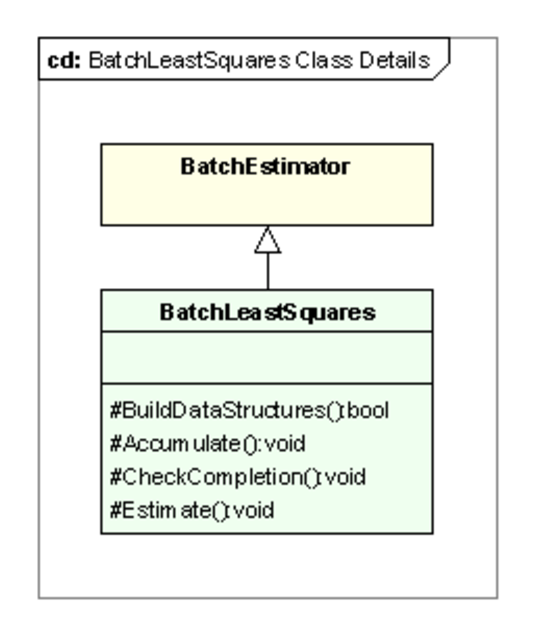
\includegraphics[scale=0.6]{Images/BatchLeastSquaresClassDetails.eps}
\caption{\label{fig:BatchLeastSquaresClass}The BatchLeastSquares Class}
\end{center}
\end{figure}

The BatchLeastSquares class, shown in Figure~\ref{fig:BatchLeastSquaresClass}, captures the mathematics of the accumulation and estimation processes.

\subsection{Key Processes}

The key processes performed by the BatchLeastSquares class are described in the parent class's text.  The BatchLeastSquares class does not provide any additional process level elements.  It does provide a specific implementation of the batch least squares algorithm, captured in the implementation of the four  abstract methods BuildDataStructures(), Accumulate(), Estimate(), and CheckCompletion().

\subsection{BatchLeastSquares Members}

\paragraph{BatchLeastSquares Attributes}

The BatchLeastSquares estimator does not require any new data members that need description at this level of the design.

\paragraph{BatchLeastSquares Methods}

\begin{itemize}
\item \textbf{virtual bool BuildDataStructures()}:  Method called by Initialize() to set up the data structures used for accumulation in the BatchLeastSquares estimator.
\item \textbf{virtual void Accumulate()}:  Collects the observed less calculated data and derivative information needed to build the normal equations.
\item \textbf{virtual void Estimate()}:  Solves the normal equations, generating the corrections that apply to the estimation state vector to construct a new estimate.
\item \textbf{virtual void CheckCompletion()}:  Checks the estimate to see if the estimation has converged or if another stopping criterion has been met.  If not, the most recent state corrections are applied to the estimation state vector.
\end{itemize}

\section{The Simulator Class}

GMAT's Simulator class is derived directly from the Solver class, and capitalizes on the state machine infrastructure provided by that class.  Simulators inherit these structures and use them to drive the simulation process. Figure~\ref{fig:SimulatorClass} shows the structure of the Simulator class, described in this section.

\begin{figure}[htbp]
\begin{center}
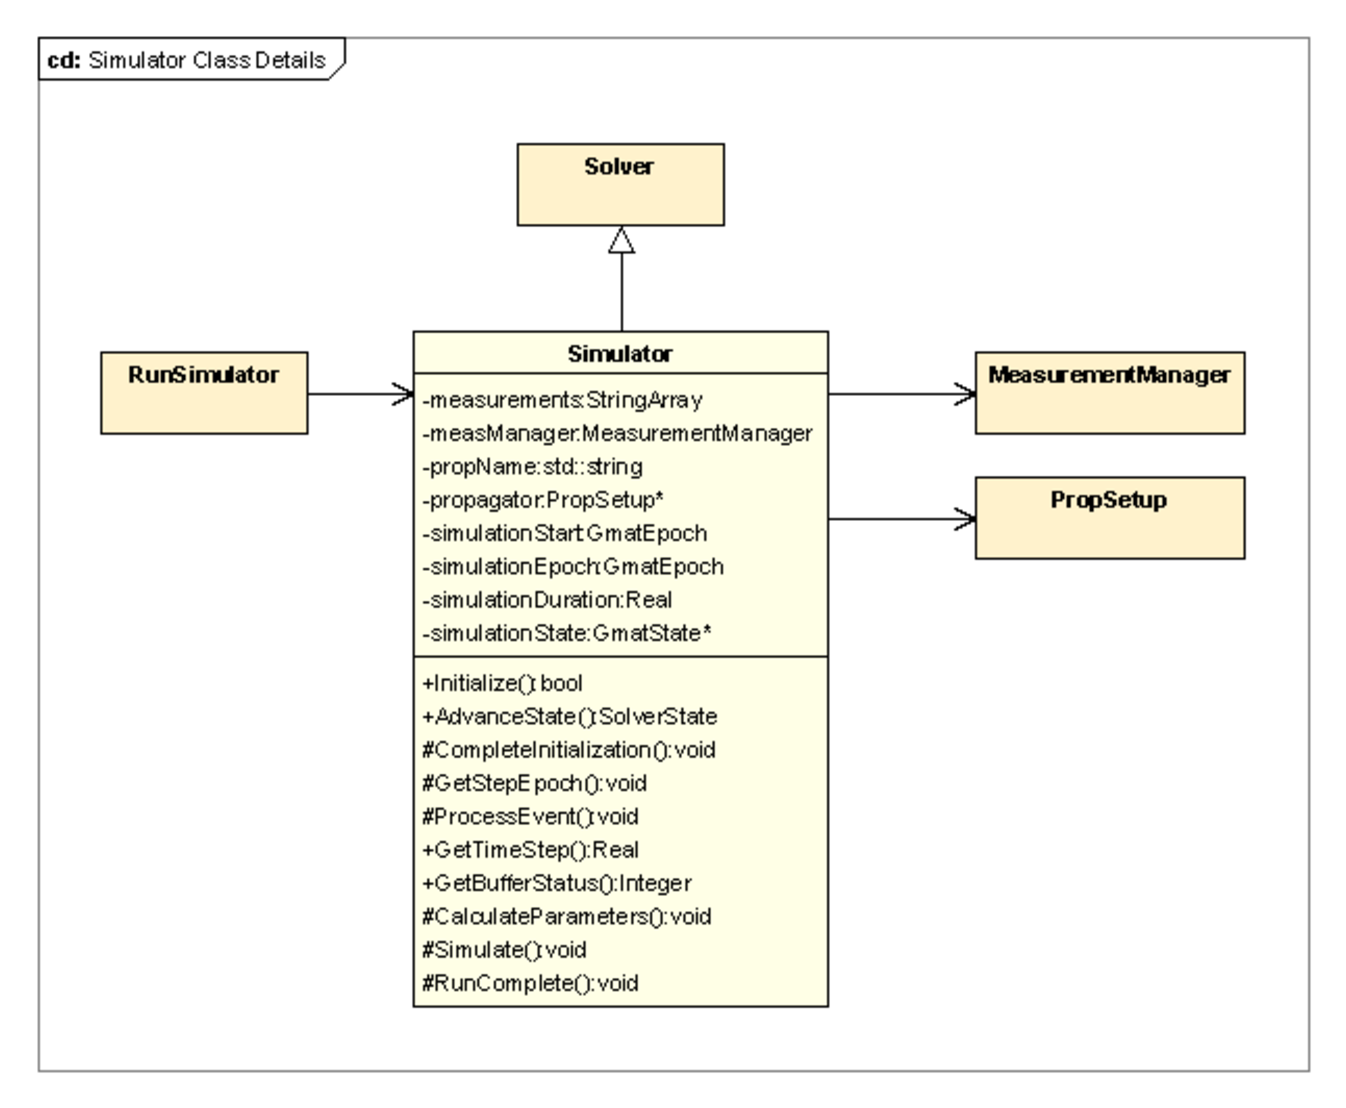
\includegraphics[scale=0.6]{Images/SimulatorClassDetails.eps}
\caption{\label{fig:SimulatorClass}The Simulator Class}
\end{center}
\end{figure}

\subsection{Key Processes}

The Simulator class has two key processes: the Initialize() method, which  initializes its management members and prepares its propagation subsystem for initialization, and the AdvanceState() method, which drives the simulation state machine.

\subsubsection{Simulator Initialization}

The initialization process manages the initialization of the MeasurementManager, PropSetup, and the referenced objects associated with these members.  The MeasurementManager initialization, described in the MeasurementManager class description, prepares the Measurement objects for use in the simulation.  The initialization for the PropSetup performs the pre-initialization steps so that the ODEModel and associated state data can be initialized at the start of the RunSimulator::Execute() call during the Mission Control Sequence run.

\subsubsection{The Simulation State Machine}

The Simulator uses six states to drive its algorithm.  These six states, shown in the bottom partition of Figure~\ref{fig:SimulatorStateMachine}, work together to simulate measurement data for a mission.

\begin{figure}[htbp]
\begin{center}
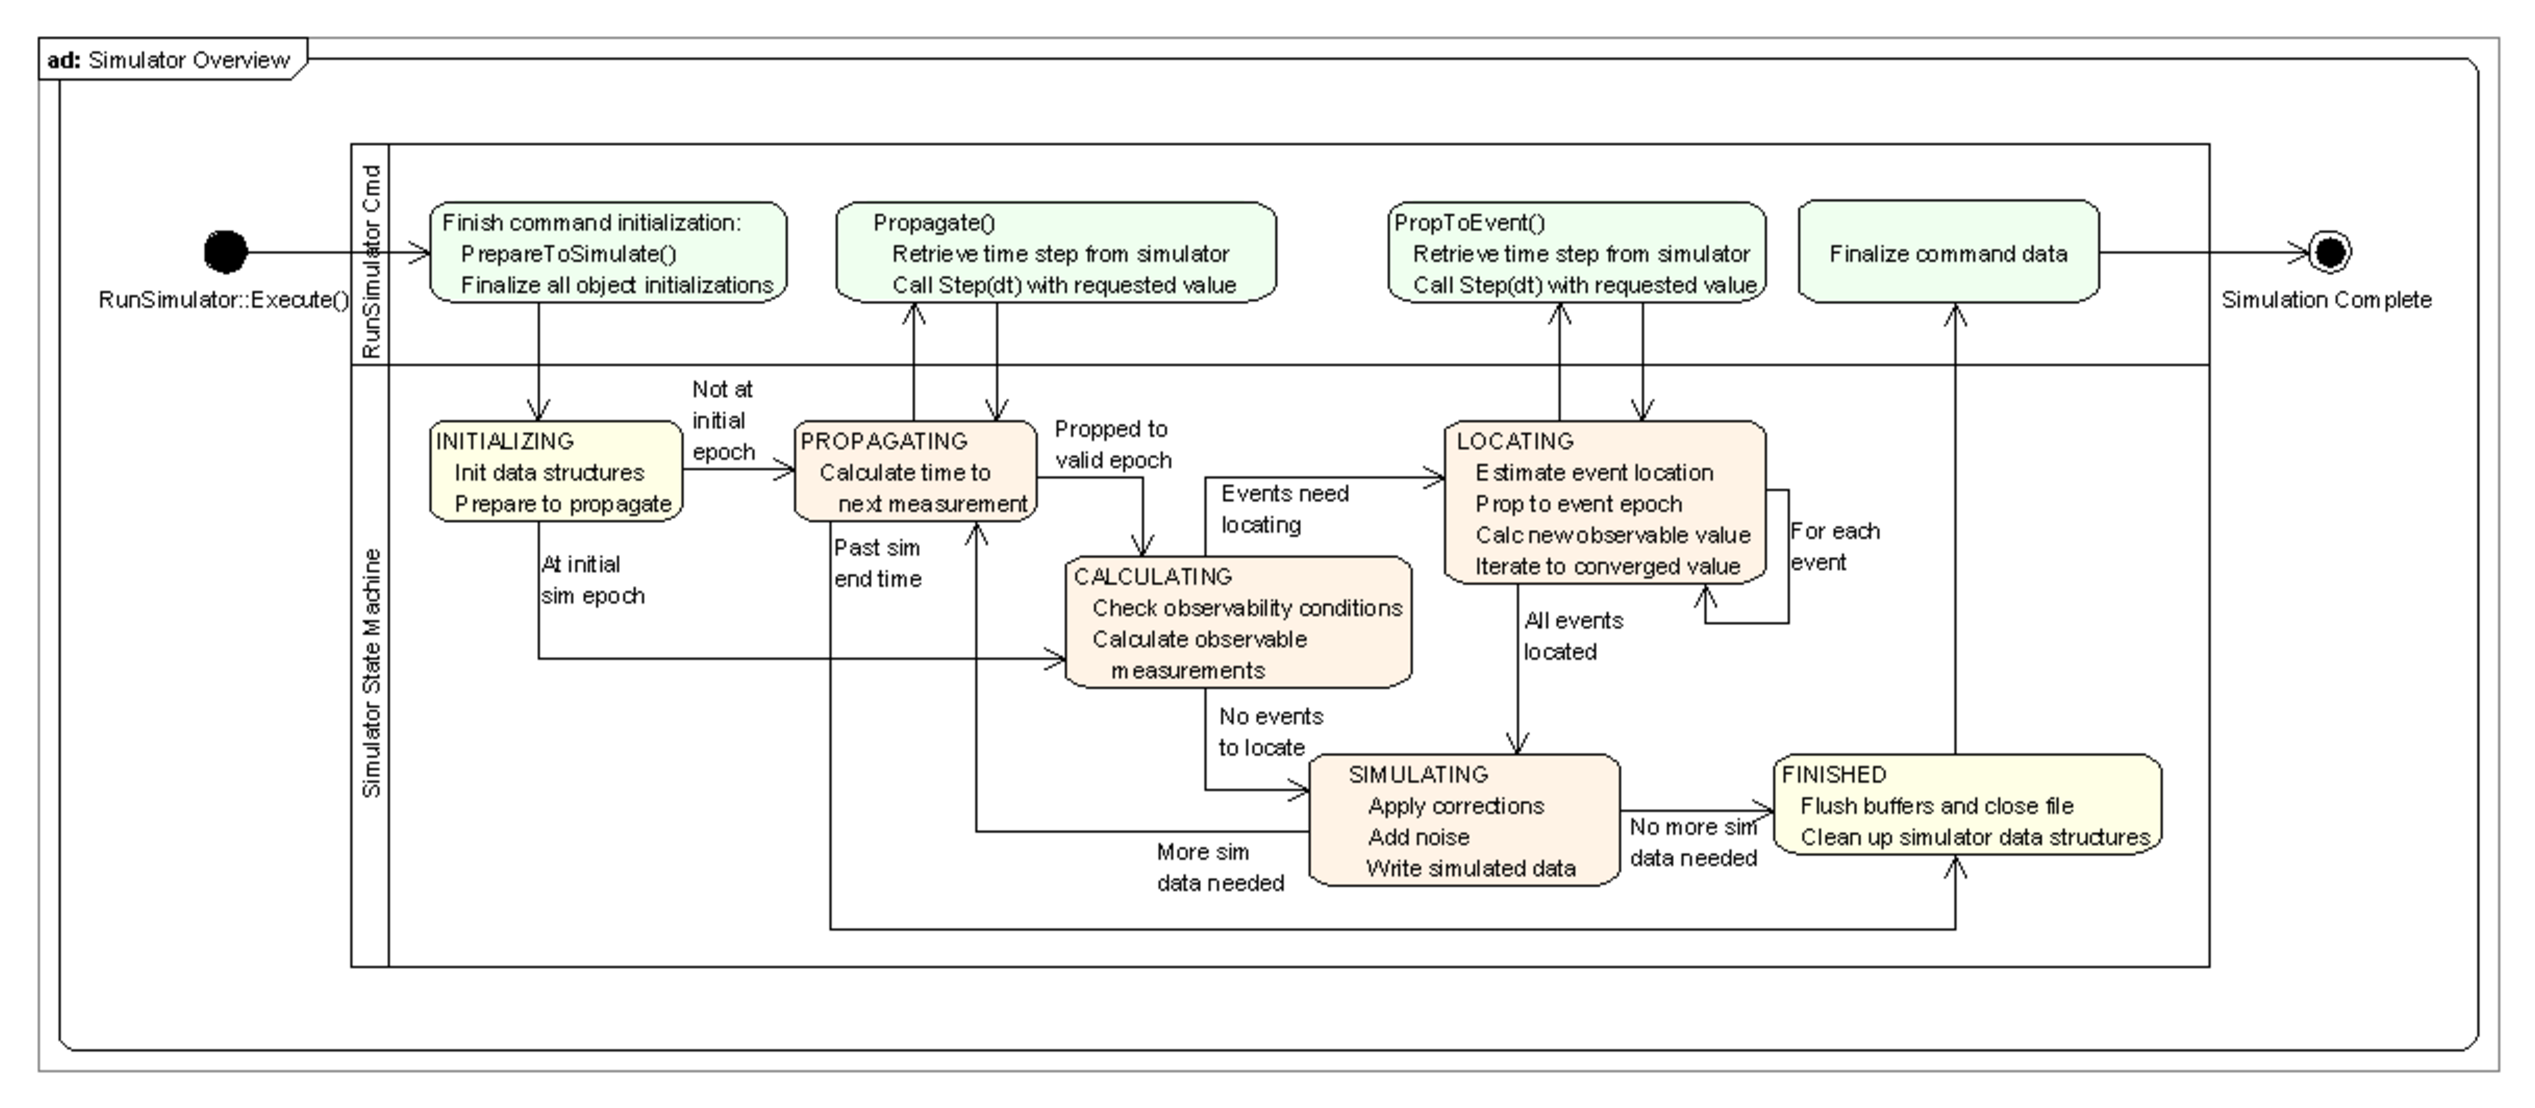
\includegraphics[scale=0.39]{Images/SimulatorOverview.eps}
\caption{\label{fig:SimulatorStateMachine}The Simulation State Machine}
\end{center}
\end{figure}

The list below describes each state of the machine, including the entry and exit conditions along with the internal actions required to move to the exit condition for the state:

\begin{description}
\item[INITIALIZING]\hspace{1pt}
\begin{itemize}
\item \textbf{Entry condition}
The INITIALIZING state is the state the Simulator takes upon completion of initialization in the Sandbox.  Upon completion of a simulation run, the Simulator returns to this state so that a subsequent call can reuse the same simulator.
\item \textbf{Actions} \textit{Method Name: CompleteInitialization()}
\begin{itemize}
\item Gather the data and fill the simulator's state.  Get current epoch from spacecraft participants, make sure all participants have the same epoch.  If not, throw an exception.
\end{itemize}
\item \textbf{Exit condition 1}:
\begin{itemize}
\item Change to PROPAGATING state if current epoch is not the simulation start epoch
\end{itemize}
\item \textbf{Exit condition 2}:
\begin{itemize}
\item Change to CALCULATING state if current epoch is the simulation start epoch
\end{itemize}
\end{itemize}
\item [PROPAGATING]\hspace{1pt}
\begin{itemize}
\item \textbf{Entry condition}:  A new observation needs to be simulated.
\item \textbf{Actions}		Method Name:  GetStepEpoch()
\begin{itemize}
\item Determine time step for propagation to the observation epoch
\item Provide time step to command for propagation on request
\item Determine if measurement for the observation has events that require propagation
\end{itemize}
\item \textbf{Exit condition 1}
\begin{itemize}
\item Propagation to the desired time has occurred
\item No unprocessed propagation events
\item Change state to CALCULATING
\end{itemize}
\item \textbf{Exit condition 2}
\begin{itemize}
\item Propagation to the desired time has occurred
\item Current epoch is past simulation end time
\item Change state to FINISHED
\end{itemize}
\end{itemize}
\item [LOCATING]\hspace{1pt}
\begin{itemize}
\item \textbf{Entry conditions}
\begin{itemize}
\item An event that requires propagation has been found
\item Resources are at a known epoch for the event, called the anchor epoch.
\end{itemize}
\item \textbf{Actions} \textit{Method Name:  ProcessEvent()}
\begin{itemize}
\item Manage the flag used to handle buffer state information
\item Calculate time step required for the event
\item Provide time step to command for propagation on request
\item Evaluate event to determine if propagation results are within tolerance
\item Iterate from time step calculation until event converges
\end{itemize}
\item \textbf{Exit condition 1}
\begin{itemize}
\item Event has converged
\item No additional events found
\item Reset state information to buffered data
\item Change state to SIMULATING
\end{itemize}
\item \textbf{Exit condition 2}
\begin{itemize}
\item Event has converged
\item Another event found
\item Change state to LOCATING and start a new iteration
\end{itemize}
\end{itemize}
\item [CALCULATING]\hspace{1pt}
\begin{itemize}
\item \textbf{Entry condition}:  Epoch is at a simulation epoch.
\item \textbf{Actions} Method Name:  CalculateParameters()
\begin{itemize}
\item Determine observability for measurements at the current epoch
\item Measurement manager gets and stores measurement values for the current epoch
\end{itemize}
\item \textbf{Exit condition 1}
\begin{itemize}
\item No measurements are observable
\item Change state to PROPAGATING
\end{itemize}
\item \textbf{Exit condition 2}
\begin{itemize}
\item At least one measurement primitive was calculated
\item No propagation is required for corrections
\item Change state to SIMULATING
\end{itemize}
\item \textbf{Exit condition 3}
\begin{itemize}
\item At least one measurement primitive was calculated
\item Corrections that require event finding were detected
\item Change state to LOCATING
\end{itemize}
\end{itemize}
\item [SIMULATING]\hspace{1pt}
\begin{itemize}
\item \textbf{Entry condition}:
All measurements and events at the current epoch have been pre-processed
\item \textbf{Actions} \textit{Method Name:  Simulate()}
\begin{itemize}
\item Apply corrections to all observable measurements
\item Tell measurement manager to write measurement data to the measurement data stream
\item Calculate the time step to the next measurement that needs to be simulated
\end{itemize}
\item \textbf{Exit condition 1}
\begin{itemize}
\item Measurement data was written to the data stream
\item Propagation time step remains within the simulation span
\item Change state to PROPAGATING
\end{itemize}
\item \textbf{Exit condition 2}
\begin{itemize}
\item Measurement data was written to the data stream
\item Propagation time step remains outside of the simulation span
\item Change state to FINISHED
\end{itemize}
\end{itemize}
\item [FINISHED]\hspace{1pt}
\begin{itemize}
\item \textbf{Entry condition}:  Simulation work finished
\item \textbf{Actions} \textit{Method Name:  RunComplete()}
\begin{itemize}
\item Clean up data structures
\item Flush and close the measurement data stream
\end{itemize}
\item \textbf{Exit condition}
\begin{itemize}
\item Change state to INITIALIZING so simulator is reentrant
\end{itemize}
\end{itemize}
\end{description}

\subsection{Simulator Members}

\paragraph{Simulator Attributes}

\begin{itemize}
\item \textbf{StringArray measurements}:  Names of the measurement models used in this simulator.
This array of names is passed to the MeasurementManager for processing.
\item \textbf{MeasurementManager measManager}:  The MeasurementManager for the simulator
\item \textbf{std::string propName}:  Name of the configured propagator used to evolve objects
during the simulation process.
\item \textbf{PropSetup *propagator}:  The propagator configured for the simulation.
\item \textbf{GmatEpoch simulationStart}:  The start epoch for the simulation.
\item \textbf{GmatEpoch simulationEpoch}:  The current epoch of the simulation.
\item \textbf{Real simulationDuration}:  The length of the simulation, in seconds.
\item \textbf{GmatState *simulationState}:  The state vector that is propagated.
\end{itemize}

\paragraph{Simulator Methods}

\begin{itemize}
\item \textbf{bool Initialize()}:  Validates reference objects and sets up all available interconnections in the simulator.
\item \textbf{Solver::SolverState AdvanceState()}:  Evaluates the status of the finite state machine and implements transitions between states.
\item \textbf{virtual void CompleteInitialization()}:  Performs the final initialization steps needed before executing the simulation.  This method is called when the finite state machine is in the INITIALIZING state, and completes the actions required to transition to the next state.
\item \textbf{virtual void GetStepEpoch()}:  Determines the time step to the next epoch for access by the RunSimulator command. This method is called when the finite state machine is in the PROPAGATING state.
\item \textbf{virtual void ProcessEvent()}:  Determines the next time step needed to manage event finding. This method is called when the finite state machine is in the LOCATING state.  It may be called repeatedly as the event finding algorithm seeks the location of one or more events.
\item \textbf{Real GetTimeStep()}:  Retrieves the most recently computed time step for use in propagation. This public method is called by the RunSimulator command to determine the desired propagation step size.
\item \textbf{Integer GetBufferingStatus()}:  Returns -1 if objects need to be restored from the buffered objects in the RunSimulator command, 0 if the buffers are not to be accessed, and +1 if the simulation objects need to be buffered.  This public method is called by the RunSimulator command to determine when buffer actions are needed.
\item \textbf{virtual void CalculateParameters()}:  Calculates measurement data in the measurement primitives. This method is called when the finite state machine is in the CALCULATING state.
\item \textbf{virtual void Simulate()}:  Calculates the fully corrected measurement values that are reported to the measurement data stream, and writes those data to the stream.  The measurement data stream can be either a file, a database, or a live data stream.  (The initial estimation builds of GMAT support the file option.)
\item \textbf{virtual void RunComplete()}:  Cleans up the data structures used during the
simulation, flushed the data buffers associated with the measurement data stream, and closes the
stream.
\end{itemize}

    \onecolumn
\chapter{Measurement Models}


\begin{equation}
    \mathcal{R}_1^{(j)} = \rho^{(m,j)}_1(t_i) +c\left(b_r^{(m)}(t_i) - b_t^{(j)}(t_t)\right) + \Delta \rho^{(j)}_{iono}(t_i) + \Delta \rho^{(j)}_{tropo}(t_i) + \sigma_{SA}^{(j)} + \sigma_n^{(j)} + b_m
\end{equation}

\begin{tabbing}
12345678912345 \= Reynolds number based on length $s$ \kill
$\mathcal{R}_1^{(j)}$         \>  One-way pseudorange measurement from transmitting \\
$$                            \> antenna $k$ on satellite $j$ to receiving antenna $m$ on satellite $n$. \\
$\rho^{(m,j)}_1(t_i)$         \>  Geometric distance between transmitting and receiveing antenntas.\\
$b_r^{(m)}(t_i)$               \> Clock bias for receiver \\
$b_t^{(j)}(t_t)$                   \>  Clock bias for transmitter\\
$\Delta \rho^{(j)}_{iono}(t_i)$    \> Correction for ionspheric delay \\
$ \Delta \rho^{(j)}_{tropo}(t_i) $ \> Correction for  Tropospheric delay\\
$\sigma_{SA}^{(j)}$                \> Error due to selective availability \\
$\sigma_n^{(j)}$                   \> Measurement noise \\
$b_m$                              \> Measurement bias \\
$t_t$                              \> Trasmission time \\
$t_r$                              \> Receive time
\end{tabbing}


The transmission time $t_t$ and the geometric range are determined
iteratively by using fixed point iteration on the following equation
%
\begin{equation}
   t_t = t_i - \frac{\rho^{(m,j)}_1(t_i) + \Delta \rho^{(j)}_{iono}(t_i) + \Delta \rho^{(j)}_{tropo}(t_i)}{c}
\end{equation}

\section{Range}

GMAT supports two primary models for spacecraft range: geometric and
radiometric. In both cases the range is a measure of the distance
between an observer and a vehicle.
 The geometric range is calculated using vector geometry and ignores signal propagation
  times and error sources.  Most, if not all, ground trackers provide the user with
  the round trip signal propagation time.  The radiometric range model uses the best
   estimate spacecraft state to determine an expected value for the round trip signal
   propagation time from observer to spacecraft and back to the observer.  Hence,
   the raw radiometric value is a measure of round trip range.

The general form of the measurement model used by GMAT is
%
\begin{equation}
   \mathcal{O}_c = \mathbf{f}_k\left(\mathbf{r}_v(t + \delta t), \dot{\mathbf{r}}_v(t + \delta t),
   \mathbf{r}_o, \dot{\mathbf{r}}_o\right) + b + \delta_a + \delta_r
\end{equation}
%
%
\begin{tabbing}[htbp!]
12345678 \= dummy line \kill
$\mathbf{f}_k$ \> The kinematic model specific to a measurement type\\
$\mathbf{r}_v$ \> Vehicle position\\
$\dot{\mathbf{r}}_v$ \> Vehicle velocity\\
$\mathbf{r}_o$ \> Observer position\\
$\dot{\mathbf{r}}_o$    \> Observer velocity\\
$t$    \> Measurement time tag\\
$b$    \> Measurement bias\\
$\delta a$    \> Atmospheric correction\\
$\delta r$     \> Relativistic correction\\
\end{tabbing}

The kinematic model for geometric range is simply
%
\begin{equation}
    \rho_c = \| \mathbf{r}_v(t) - \mathbf{r}_g(t)\|
\end{equation}
%

The kinematic model for radiometric two way range is
%
\begin{equation}
     \rho_c= \frac{1}{2}\left(\| \mathbf{r}_v(t_{v}) -  \mathbf{r}_g(t_{gt})  \| +
      \| \mathbf{r}_v(t_{v}) -  \mathbf{r}_g(t_{gt})  \|\right) \label{Eq:ExpectedTwoWayRange}
\end{equation}
%
where
%
\begin{tabbing}[htbp!]
12345678 \= dummy line \kill
$t_{gt}$ \> Time the uplink signal is transmitted from ground station\\
$t_{vr}$ \> Time the uplink signal is received at vehicle\\
$t_{vt}$ \> Time the downlink signal is transmitted from vehicle\\
$t_{gr}$ \> Time the downlink signal is received at ground station\\
$t_u$    \> Uplink propagation time, ( $t_{vr}$ - $t_{gt}$ )\\
$t_d$    \> Downlink propagation time, ( $t_{vt}$ - $t_{gr}$ )\\
$\rho_u$    \> Uplink distance\\
$\rho_d$    \> Downlink distance\\
$d_T$     \> Distance traveled by vehicle during transponder delay\\
$\mathbf{r}_v(t)$ \> Position of vehicle at time $t$\\
$\mathbf{r}_t(t)$ \> Position of transmitter at time $t$\\
$\mathbf{r}_r(t)$ \> Position of receiver at time $t$\\
$t$           \>  time of geometric range measurement \\
$\delta T$  \>  Vehicle's transponder delay time\\
$\delta t_a$  \>  Atmospheric delays\\
$\delta t_r$  \>  Relativistic effects\\
\end{tabbing}
%

The radiometric model is derived from the measurement geometry shown
in Fig.~\ref{Fig:RangeMeasurement}. We see that the total signal
propagation time is the sum of three times, the uplink
 signal propagation time, $t_u$, the transponder delay time, $\delta T$, and
 the downlink propagation time, $t_d$.  Hence, the observed value for signal propagation time, $t_o$, is
%
\begin{equation}
     \Delta t_o = t_{gr} - t_{gt} = t_u + \delta T + t_d
\end{equation}
%
\begin{figure}[htbp!]
    \begin{center}
    \begin{picture}(270,215)
    \special{psfile= RangeMeasurement.eps
    hscale= 75 vscale= 75 hoffset = -85 voffset = -270}
        \makebox(175,295){ $\mathbf{r}_v(t_{vr})$}
        \makebox(-25,290){ $\mathbf{r}_v(t_{vt})$}
        \makebox(85,290){ $\rho_d$}
        \makebox(-100,90){ $\mathbf{r}_g(t_{gr})$}
        \makebox(-460,90){ $\mathbf{r}_g(t_{gt})$}
        \makebox(-485,290){ $\rho_u$}
        \makebox(-305,390){ $d_T$}
    \end{picture}
    \end{center}
    \vspace{0.2 in}
    \label{Fig:RangeMeasurement}
    \caption{ Geometry of Radiometric Range Measurement}
\end{figure}
%
The elapsed time is converted to a measure of the average range
using
%
\begin{equation}
     \rho_o = \frac{c}{2}\Delta t_o
\end{equation}
%
The computed elapsed time is rigorously expressed as
%
\begin{equation}
    \Delta t_c = \frac{1}{c}\| \mathbf{r}_v(t_{vr}) -  \mathbf{r}_g(t_{gt})  \| +
    \frac{1}{c}\| \mathbf{r}_v(t_{vt}) -  \mathbf{r}_g(t_{gr})  \| + \delta T
\end{equation}
%
Assuming that the transponder delay is modelled as a measurement
bias we can write $ t_{vr} = t_{vt} = t_v$ and convert the computed
round trip time to average range:
%
\begin{equation}
     \rho_c= \frac{1}{2}\left(\| \mathbf{r}_v(t_v) -  \mathbf{r}_g(t_{gt})  \| +
      \| \mathbf{r}_v(t_v) -  \mathbf{r}_g(t_{gr})  \|\right) \label{Eq:MeasuredTwoWayRange}
\end{equation}
%
To solve Eq.~\ref{Eq:MeasuredTwoWayRange}, we must know  $t_{v}$.
For applications
 that do not require high accuracy we can approximate $t_v$ as we describe below.
  For higher fidelity applications we must solve for the uplink and downlink
  propagation times using two iterative processes.  The downlink signal propagation
  time is calculated using the following fixed point iteration on the following equation:
%
\begin{equation}
     \delta t_d^{i+1} = \frac{1}{c}\| \mathbf{r}_v( t - t_d^{i}) - \mathbf{r}_g(t)   \|
\end{equation}
%
The uplink propagation time is calculated using fixed point
iteration on
%
\begin{equation}
     \delta t_u^{i+1} = \frac{1}{c}\| \mathbf{r}_v( t - t_d) - \mathbf{r}_g(t - t_d - t_u^{i} )   \|
\end{equation}
%

\begin{eqnarray}
     \frac{\partial \rho_c (t)}{\partial \mathbf{r}_v(t_v)} &=& \frac{1}{2\rho_u\rho_d}
     \left( \rho_d(\mathbf{r}_v^T(t_v) - \mathbf{r}_T^T(t_{gt}) + \rho_u(\mathbf{r}_v^T(t_v) - \mathbf{r}_R^T(t_{gr}  ) \right)\\
     %
     \frac{\partial \rho_c (t)}{\partial \dot{\mathbf{r}}_v(t_v)} &=& \mathbf{0}_{1x3}
\end{eqnarray}


\chapter{High-level Architectural Design}
    \section{State Vector Overview}

GMAT requires two distinct types of state information when solving estimation problems.  The
estimators operate on an estimation state vector containing the elements that are estimated or
considered during the estimation process.  That process requires a mechanism that models the
evolution of elements of the estimation state vector -- and, potentially, other model elements --
over time. These elements are assembled into a propagation state vector designed to facilitate fast
numerical evolution from one epoch to another.

State vectors in GMAT provide the following capabilities:

\begin{itemize}
\item Specify the values of the represented parameters at an epoch
\item Provide an extendable structure for state data
\item Identify each element by type for the purposes of mapping to and from objects
\item Identify each element by name so that user friendly vector descriptions can be generated
\item Allow access to the raw state vector for direct manipulation to meet performance requirements
\item Provide mechanisms to manipulate the vector element by element or as collections of elements
\item Allow a handshake mechanism so that the system components that manipulate the state vector
can map the elements onto other system components
\item Make decomposition of the state vector into subvectors simple to manage in the code
\end{itemize}

These derived requirements drive the design for the class structure used to model all GMAT state
vectors.  Customization of the state vector for the specific needs of the other elements of GMAT is
performed using a state vector manager.  The state vector manager provides the interfaces required
by the propagation and estimation subsystems to synchronize the state data with GMAT's objects, and
with the numerical engines controlled by those subsystems.

The state manager base class contains the structures and basic interfaces used to provide these
features:

\begin{itemize}
\item Manage a state vector
\item Copy object data into and out of the state vector
\item Map vector elements to their mathematical models
\item Ensure data consistency for the state vector
\item Provides a generic interface used by subclasses to construct state manipulation components
like derivative models and estimation state manipulators
\end{itemize}




<OTHER TEXT STILL IN THE WORKS>

The following sections describe the classes, derived from GMAT's base state representation, that
are used to model the estimation state vector and the propagation state vector.
    \section{ Estimation State Vector }

    \section{Propagation State Vector } 

    \section{Estimators}

    \section{Partial Derivatives}

    \section{Measurement Processing}

    \section{Commands}

Users use GMAT's command subsystem to design the mission timeline that they would like to model.
In GMAT, this timeline is called the mission control sequence.  It consists of a list of
instructions defining the time ordered sequence of actions that occur to model the mission GMAT is
simulating.

The incorporation of estimation into GMAT necessitates extension of the mission control sequence to
accommodate the instructions required to perform estimation specific tasks.  In addition, some of
the existing commands in GMAT need to be modified to neet the needs of the estimation process.

GMAT will include four new commands tailored to estimation: RunEstimator, RunSimulator, Estimate,
and EndEstimate.  The Propagate command will be extended work with the expanded capabilities of the
state vector, described earlier in this chapter, and to function correctly when included as part of
an estimation control sequence defined by the Estimate and EndEstimate commands.

Many estimation tasks can be performed through simple propagation of the estimation state vector
and related quantities, with no events or state changes dictated outside of the control provided by
the estimator.  GMAT provides two commands designed to run estimation in the mission control
sequence using this paradigm: the RunEstimator and the RunSimulator commands.  Like the
Propagate command, these commands use GMAT's propagation subsystem to perform numerical or analytic
propagation of the evolving elements of a state vector.  Figure~\ref{fig:PropEnabledCommands} shows
the highest level view of the lifetime of these commands.

\begin{figure}[htb]
\centering
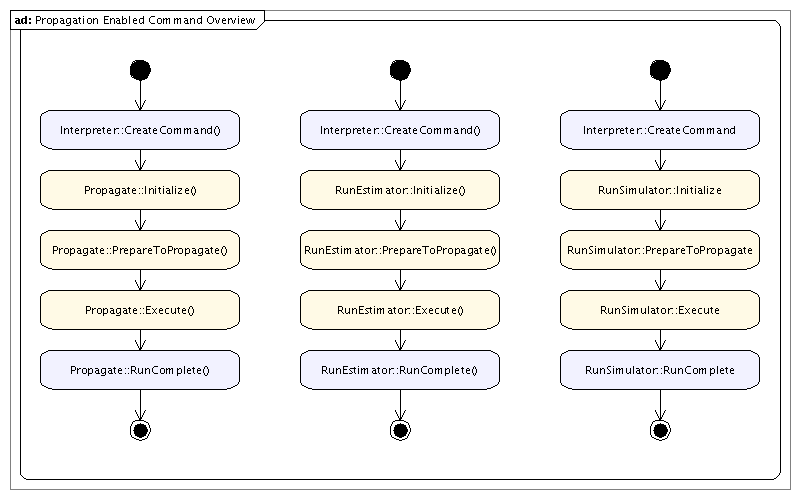
\includegraphics[400,250]{Images/PropagationEnabledCommandOverview.png}
\caption{Commands that Propagate Directly}
\label{fig:PropEnabledCommands}
\end{figure}

Each command is created as a stand alone entity by an interpreter when a script calling for the
command is opened.  When a user tells GMAT to run the script, the elements constructed by the
interpreter are passed into the Sandbox responsible for the run.  This object passing includes
insertion of the mission control sequence containing the propagation enabled command into the
Sandbox and setting of the object stores and environment data on the commands. The next call to the
command is a call to its Initialize() method, which ensures that all of the necessary elements
needed by the command exist, and sets pointers to those elements.  When the command fired in the
mission control sequence, the first phase of execution is a call to the command's
PrepareToPropagate() method, which constructs and populates the state vectors used in the execution
of the command.  Following this call, the command is executed, and runs to completion.  When the
mission control sequence has finished running, the RunComplete method is called on teh command,
completing the sequence of actions taken on the command.

The Estimate command provides a more customizable approach for users that need to include more
complicated control flow in the estimation process.  An Estimate command does not propagate
directly.  Instead, it defines the start of an estimation sequence designed to model the portion of
the mission control sequence that is being estimated.  The estimation sequence is terminated with
an EndEstimate command. Users define the timeline for the estimation process by adding commands
between teh Estimate command and the EndEstimate command.  This command pair functions similarly to
other command pairs found in GMAT: the Estimate command manages an estimator and a control
sequence, and drives the estimator state machine and control sequence in a synchronized fashion in
order to solve the estimation process.  Figure~\ref{fig:EstimateCommandOverview} shows the high
level view of the processes performed over the life of an Estimate/EndEstimate command pair.

\begin{figure}[htbp]
\centering
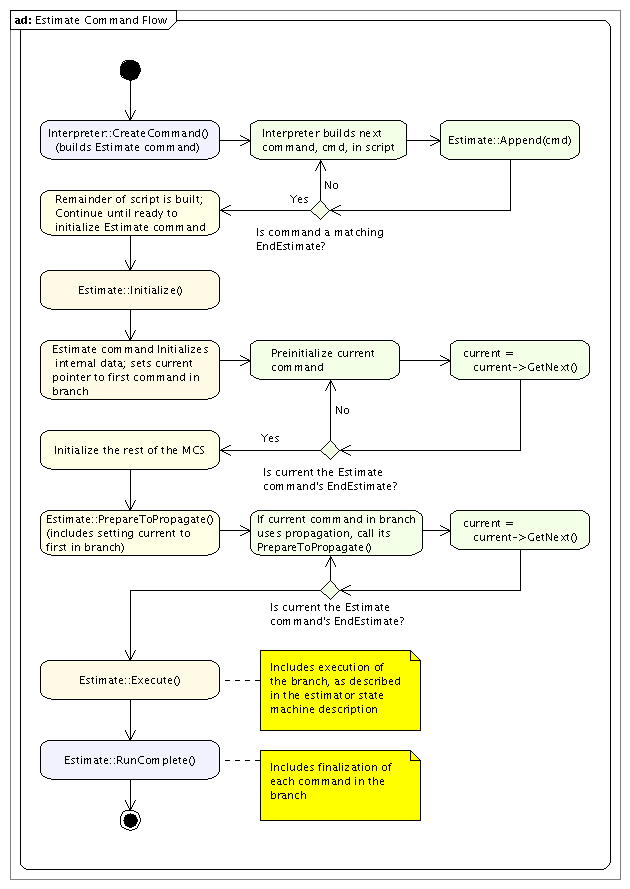
\includegraphics[315,445]{Images/EstimateCommandFlow.png}
\caption{Estimation with an Estimation Control Sequence}
\label{fig:EstimateCommandOverview}
\end{figure}



\subsection{Estimation Commands that Propagate}

\subsubsection{RunEstimator}

\subsubsection{RunSimulator}



\subsection{Estimate and EndEstimate}

\subsection{Propagate}

The Propagate command is used to control both fine grained and large scale evolution of mission
elements in GMAT.

\chapter{Questions and Thoughts}

This chapter is for capturing questions and unaddressed issues while
we work on this document.

\begin{itemize}
     \item If a user has a measurement data file that has data for
     multiple spacecraft and multiple ground stations, how can the
     specify to only use a subset of the data.  Matt suggested using
     an Exclude field on a measurement.
\end{itemize}





\begin{thebibliography}{9}% maximum number of references (for label width)

   \bibitem{GTDS:89} Long, A., and Cappellari, J. O. \emph{et al}, ``Goddard Trajectory Determination System
    Mathematical Theory, Revision 1,"  \emph{NASA Goddard Space Flight Center}, Greenbelt, MD, 1989.

    \bibitem{DatSim:08} Long, A., \emph{et al}, ``User Guide and Mathematical Specifications for the Measurement Data Simulation Program
    Release 2.11,"  \emph{NASA Goddard Space Flight Center}, Greenbelt, MD, Sept., 2008.

\end{thebibliography}

\end{document}

%------------------------------------------------------------
%-----------------Part I:  Mathematical Specifications-------
%------------------------------------------------------------
\onecolumn
\chapter{Measurement Models}


\begin{equation}
    \mathcal{R}_1^{(j)} = \rho^{(m,j)}_1(t_i) +c\left(b_r^{(m)}(t_i) - b_t^{(j)}(t_t)\right) + \Delta \rho^{(j)}_{iono}(t_i) + \Delta \rho^{(j)}_{tropo}(t_i) + \sigma_{SA}^{(j)} + \sigma_n^{(j)} + b_m
\end{equation}

\begin{tabbing}
12345678912345 \= Reynolds number based on length $s$ \kill
$\mathcal{R}_1^{(j)}$         \>  One-way pseudorange measurement from transmitting \\
$$                            \> antenna $k$ on satellite $j$ to receiving antenna $m$ on satellite $n$. \\
$\rho^{(m,j)}_1(t_i)$         \>  Geometric distance between transmitting and receiveing antenntas.\\
$b_r^{(m)}(t_i)$               \> Clock bias for receiver \\
$b_t^{(j)}(t_t)$                   \>  Clock bias for transmitter\\
$\Delta \rho^{(j)}_{iono}(t_i)$    \> Correction for ionspheric delay \\
$ \Delta \rho^{(j)}_{tropo}(t_i) $ \> Correction for  Tropospheric delay\\
$\sigma_{SA}^{(j)}$                \> Error due to selective availability \\
$\sigma_n^{(j)}$                   \> Measurement noise \\
$b_m$                              \> Measurement bias \\
$t_t$                              \> Trasmission time \\
$t_r$                              \> Receive time
\end{tabbing}


The transmission time $t_t$ and the geometric range are determined
iteratively by using fixed point iteration on the following equation
%
\begin{equation}
   t_t = t_i - \frac{\rho^{(m,j)}_1(t_i) + \Delta \rho^{(j)}_{iono}(t_i) + \Delta \rho^{(j)}_{tropo}(t_i)}{c}
\end{equation}

\section{Range}

GMAT supports two primary models for spacecraft range: geometric and
radiometric. In both cases the range is a measure of the distance
between an observer and a vehicle.
 The geometric range is calculated using vector geometry and ignores signal propagation
  times and error sources.  Most, if not all, ground trackers provide the user with
  the round trip signal propagation time.  The radiometric range model uses the best
   estimate spacecraft state to determine an expected value for the round trip signal
   propagation time from observer to spacecraft and back to the observer.  Hence,
   the raw radiometric value is a measure of round trip range.

The general form of the measurement model used by GMAT is
%
\begin{equation}
   \mathcal{O}_c = \mathbf{f}_k\left(\mathbf{r}_v(t + \delta t), \dot{\mathbf{r}}_v(t + \delta t),
   \mathbf{r}_o, \dot{\mathbf{r}}_o\right) + b + \delta_a + \delta_r
\end{equation}
%
%
\begin{tabbing}[htbp!]
12345678 \= dummy line \kill
$\mathbf{f}_k$ \> The kinematic model specific to a measurement type\\
$\mathbf{r}_v$ \> Vehicle position\\
$\dot{\mathbf{r}}_v$ \> Vehicle velocity\\
$\mathbf{r}_o$ \> Observer position\\
$\dot{\mathbf{r}}_o$    \> Observer velocity\\
$t$    \> Measurement time tag\\
$b$    \> Measurement bias\\
$\delta a$    \> Atmospheric correction\\
$\delta r$     \> Relativistic correction\\
\end{tabbing}

The kinematic model for geometric range is simply
%
\begin{equation}
    \rho_c = \| \mathbf{r}_v(t) - \mathbf{r}_g(t)\|
\end{equation}
%

The kinematic model for radiometric two way range is
%
\begin{equation}
     \rho_c= \frac{1}{2}\left(\| \mathbf{r}_v(t_{v}) -  \mathbf{r}_g(t_{gt})  \| +
      \| \mathbf{r}_v(t_{v}) -  \mathbf{r}_g(t_{gt})  \|\right) \label{Eq:ExpectedTwoWayRange}
\end{equation}
%
where
%
\begin{tabbing}[htbp!]
12345678 \= dummy line \kill
$t_{gt}$ \> Time the uplink signal is transmitted from ground station\\
$t_{vr}$ \> Time the uplink signal is received at vehicle\\
$t_{vt}$ \> Time the downlink signal is transmitted from vehicle\\
$t_{gr}$ \> Time the downlink signal is received at ground station\\
$t_u$    \> Uplink propagation time, ( $t_{vr}$ - $t_{gt}$ )\\
$t_d$    \> Downlink propagation time, ( $t_{vt}$ - $t_{gr}$ )\\
$\rho_u$    \> Uplink distance\\
$\rho_d$    \> Downlink distance\\
$d_T$     \> Distance traveled by vehicle during transponder delay\\
$\mathbf{r}_v(t)$ \> Position of vehicle at time $t$\\
$\mathbf{r}_t(t)$ \> Position of transmitter at time $t$\\
$\mathbf{r}_r(t)$ \> Position of receiver at time $t$\\
$t$           \>  time of geometric range measurement \\
$\delta T$  \>  Vehicle's transponder delay time\\
$\delta t_a$  \>  Atmospheric delays\\
$\delta t_r$  \>  Relativistic effects\\
\end{tabbing}
%

The radiometric model is derived from the measurement geometry shown
in Fig.~\ref{Fig:RangeMeasurement}. We see that the total signal
propagation time is the sum of three times, the uplink
 signal propagation time, $t_u$, the transponder delay time, $\delta T$, and
 the downlink propagation time, $t_d$.  Hence, the observed value for signal propagation time, $t_o$, is
%
\begin{equation}
     \Delta t_o = t_{gr} - t_{gt} = t_u + \delta T + t_d
\end{equation}
%
\begin{figure}[htbp!]
    \begin{center}
    \begin{picture}(270,215)
    \special{psfile= RangeMeasurement.eps
    hscale= 75 vscale= 75 hoffset = -85 voffset = -270}
        \makebox(175,295){ $\mathbf{r}_v(t_{vr})$}
        \makebox(-25,290){ $\mathbf{r}_v(t_{vt})$}
        \makebox(85,290){ $\rho_d$}
        \makebox(-100,90){ $\mathbf{r}_g(t_{gr})$}
        \makebox(-460,90){ $\mathbf{r}_g(t_{gt})$}
        \makebox(-485,290){ $\rho_u$}
        \makebox(-305,390){ $d_T$}
    \end{picture}
    \end{center}
    \vspace{0.2 in}
    \label{Fig:RangeMeasurement}
    \caption{ Geometry of Radiometric Range Measurement}
\end{figure}
%
The elapsed time is converted to a measure of the average range
using
%
\begin{equation}
     \rho_o = \frac{c}{2}\Delta t_o
\end{equation}
%
The computed elapsed time is rigorously expressed as
%
\begin{equation}
    \Delta t_c = \frac{1}{c}\| \mathbf{r}_v(t_{vr}) -  \mathbf{r}_g(t_{gt})  \| +
    \frac{1}{c}\| \mathbf{r}_v(t_{vt}) -  \mathbf{r}_g(t_{gr})  \| + \delta T
\end{equation}
%
Assuming that the transponder delay is modelled as a measurement
bias we can write $ t_{vr} = t_{vt} = t_v$ and convert the computed
round trip time to average range:
%
\begin{equation}
     \rho_c= \frac{1}{2}\left(\| \mathbf{r}_v(t_v) -  \mathbf{r}_g(t_{gt})  \| +
      \| \mathbf{r}_v(t_v) -  \mathbf{r}_g(t_{gr})  \|\right) \label{Eq:MeasuredTwoWayRange}
\end{equation}
%
To solve Eq.~\ref{Eq:MeasuredTwoWayRange}, we must know  $t_{v}$.
For applications
 that do not require high accuracy we can approximate $t_v$ as we describe below.
  For higher fidelity applications we must solve for the uplink and downlink
  propagation times using two iterative processes.  The downlink signal propagation
  time is calculated using the following fixed point iteration on the following equation:
%
\begin{equation}
     \delta t_d^{i+1} = \frac{1}{c}\| \mathbf{r}_v( t - t_d^{i}) - \mathbf{r}_g(t)   \|
\end{equation}
%
The uplink propagation time is calculated using fixed point
iteration on
%
\begin{equation}
     \delta t_u^{i+1} = \frac{1}{c}\| \mathbf{r}_v( t - t_d) - \mathbf{r}_g(t - t_d - t_u^{i} )   \|
\end{equation}
%

\begin{eqnarray}
     \frac{\partial \rho_c (t)}{\partial \mathbf{r}_v(t_v)} &=& \frac{1}{2\rho_u\rho_d}
     \left( \rho_d(\mathbf{r}_v^T(t_v) - \mathbf{r}_T^T(t_{gt}) + \rho_u(\mathbf{r}_v^T(t_v) - \mathbf{r}_R^T(t_{gr}  ) \right)\\
     %
     \frac{\partial \rho_c (t)}{\partial \dot{\mathbf{r}}_v(t_v)} &=& \mathbf{0}_{1x3}
\end{eqnarray}


\end{document}
